%!TEX program=xelatex
\documentclass[14pt,a4paper]{article}

\usepackage[UTF8]{ctex}
\usepackage[T1]{fontenc}
\usepackage{textcomp}
\usepackage{enumerate}
\usepackage{amsmath, amssymb, amsthm}
\usepackage{mathdots}
% Hyperlinks
\usepackage{hyperref}
\hypersetup{colorlinks=true,
			linkcolor=blue,
			anchorcolor=blue,
			citecolor=cyan}
% figure support
\usepackage{float}
\usepackage{import}
\usepackage{xifthen}
\usepackage{pdfpages}

% Theorem-like statements
% Theorem
\theoremstyle{plain}
\newtheorem{thm}{Theorem}[section]
\newtheorem*{nnt}{Theorem}
% Definition
\theoremstyle{definition}
\newtheorem*{dfn}{Definition}
% Remark
\theoremstyle{remark}
\newtheorem{rmk}{Remark}[section]
\newtheorem*{nnr}{Remark}
% Lemma
\theoremstyle{plain}
\newtheorem{lem}[thm]{Lemma}
\newtheorem*{nnl}{Lemma}
% Corollary
\theoremstyle{plain}
\newtheorem{cor}[thm]{Corollary}
\newtheorem*{nnc}{Corollary}
% Proposition 
\theoremstyle{plain}
\newtheorem{prop}[thm]{Proposition}
\newtheorem*{nnp}{Proposition}
% Axiom
\theoremstyle{definition}
\newtheorem{axm}{Axiom}[section]
\newtheorem*{nnax}{Axiom}
% Algorithm 
\theoremstyle{remark}
\newtheorem{alg}{Algorithm}[section]
\newtheorem*{nnal}{Algorithm}

% Title
\title{AUTO3001B 自动控制原理B 笔记}
\author{H. Luan}
\date{2020年3月}

\numberwithin{equation}{section}

\begin{document}
	\maketitle
	\newpage
	\tableofcontents %Contents
	\newpage

	\setcounter{section}{-1}
	\section{绪论}
	\label{sec:绪论}

		\subsection{控制系统设计与综合}%
		\label{sub:控制系统设计与综合}
		
			
			\begin{itemize}
				\item 当系统不能满足希望的性能或不能完成所规定的任务时,需要对系统进行干预、调节或控制来改变原系统,使改变后的系统满足所规定的任务或性能要求 ------  这一完整过程称为\emph{控制系统设计} 或控制系统综合。 
				\item 系统模型
					\begin{table}[h]
						\centering
						\begin{tabular}{c|p{90pt}|c}
							 & 连续时间系统 & 离散时间系统 \\
							 \hline
							传递函数模型 & 基于Bode图的频域校正、基于根轨迹的设计方法 & 基于Bode图的频域校正模拟化设计\\
							\hline 
							状态空间模型 & \multicolumn{2}{c}{极点配置方法} \\
							\hline
							非线性系统 &\multicolumn{2}{c}{描述函数法} \\
						\end{tabular}
						\caption{系统模型与分类}
					\end{table}
			\end{itemize}

			\paragraph{控制系统组成}%
			\label{par:控制系统组成}
			
				\ 
				\begin{itemize}
					\item 不可变部分
						\begin{itemize}
							\item 执行机构
							\item 功率放大器
							\item 测量元件
							\item 被控对象
						\end{itemize}
					\item 可变部分:校正装置
						\begin{itemize}
							\item 为使系统达到某种动态及静态指标要求,加入一些参数可根据需要改变的装置,该装置能改善系统性能使系统得到校正。
							\item 校正装置的选择及其参数整定的过程称为自动系统的校正。
						\end{itemize}

				\end{itemize}


		\subsection{校正方式}%
		\label{sub:校正方式}

			用于传递函数模型。
			\begin{enumerate}
				\item 串联校正
					\begin{itemize}
						\item 主要问题:对参数变化的敏感性较强
						\item 优点:从设计到具体实现比较简单,在设计中最常使用
					\end{itemize}
				\item 并联(反馈)校正
					\begin{itemize}
						\item 反馈信号由高功率点传向低功率点,一般无需附加放大器
						\item 选在合适反馈增益,可使校正后的系统性能主要取决于校正装置,而与反馈校正装置所包围的系统固有部分(被校正的环节)特性无关
						\item 优点:可抑制系统参数波动及非线性因素对系统性能的影响
						\item 设计相对较为复杂
					\end{itemize}
				\item 前馈校正
				\item 复合校正
			\end{enumerate}
			
		\subsection{控制方式}%
		\label{sub:控制方式0}

			用于状态空间模型。
			\begin{equation*}
			\begin{cases}
				\begin{aligned}
				\dot x = Ax + Bu \\
				y = Cx + Du
				\end{aligned}  
			\end{cases}
			.\end{equation*} 
			
			\subsubsection{状态反馈}%
			\label{ssub:状态反馈}
			
				\[
				u = Kx + Gr	
				.\]
				状态反馈用尽了控制系统内的全部信息,理论上控制性能应最强。

			\subsubsection{输出反馈至参考输入}%
			\label{ssub:输出反馈至参考输入}
			
				\[
				u = Fy + Gr
				.\] 
				\begin{itemize}
					\item 不能获取所有状态变量信息时可以采用
				\end{itemize}

			\subsubsection{输出反馈至状态微分}%
			\label{ssub:输出反馈至状态微分}
			
				\[
				\begin{split}
					\dot x &= Ax + u \\
					u &= Hy + Br
				\end{split}
				.\] 

			\subsubsection{动态补偿器}%
			\label{ssub:动态补偿器}

				\[
				\begin{cases}
					\dot z = Fz + Hy + Lr  \\
					u = Nz + My + Gr
				\end{cases}
				.\]
				\begin{itemize}
					\item 一类特殊的动态补偿器:基于状态观测器的反馈
				\end{itemize}

		\subsection{先修课程}%
		\label{sub:先修课程}
		
			\begin{enumerate}
				\item 自控理论A
					\begin{itemize}
						\item 时域响应
						\item 频率特性
						\item Nyquist图、Bode图
						\item Nyquist判据
					\end{itemize}
				\item 线性代数
					\begin{itemize}
						\item 线性方程有解的秩条件
						\item Cayley-Hamilton定理
					\end{itemize}
				\item 常微分方程
			\end{enumerate}	
	

	\newpage
	\section{控制系统的性能指标}%
	\label{sec:控制系统的性能指标}
	
		\subsection{稳定裕度}%
		\label{sub:稳定裕度}

			稳定是控制系统的基本要求。系统参数发生变化时,系统可能从稳定变为不稳定。在控制系统稳定的基础上,进一步表征其稳定程度高低的概念,是控制系统的相对稳定性。相对稳定性通过 \emph{稳定裕度} 定量描述,其包括 \emph{相位(相角)裕度} 和 \emph{幅值裕度}。


			\begin{dfn}[剪切频率]  
			\label{dfn:剪切频率}
			开环频率特性$G(\mathrm{j} \omega)H(\mathrm{j} \omega)$在Nyquist图上与单位圆相交处的角频率$\omega_c$,i.e. 
			 \[
				 \left| G(\mathrm{j} \omega_c)H(\mathrm{j}\omega_c ) \right| = 1
			.\] 
			\end{dfn} 

			\begin{dfn}[相角裕度]  
			\label{dfn:相角裕度}
			在$\omega = \omega_c$时,开环相频特性$\angle [G(\mathrm j \omega_c)H(\mathrm j\omega_c)]$ 与$-180^\circ$ 的相角差$\gamma$ 称为相角裕度, i.e.  
			\[
				\gamma = \pi + \angle [G(\mathrm{j} \omega_c)H(\mathrm j \omega_c)] 
			.\] 
			\end{dfn} 
			\begin{rmk}[相角裕度的物理意义]  
			\label{rmk:相角裕度的物理意义}
			如果在剪切频率$\omega_c$ 处再使相位滞后$\gamma$ ,闭环系统即达到临界稳定状态(Nyquist曲线过$(-1,\mathrm{j} 0)$ 点)。相角裕度越大,系统稳定程度越高。
			\end{rmk}

			\begin{dfn}[相位穿越频率]  
			\label{dfn:相位穿越频率}
				开环频率特性相角为$-180^\circ$ 时所对应的角频率,i.e. 
				\[
					\angle G(\mathrm{j} \omega_g)H(\mathrm{j} \omega_g) = -\pi
				.\] 
			\end{dfn} 


			\begin{dfn}[幅值裕度]  
			\label{dfn:幅值裕度}
				在$\omega=\omega_g$ 时,开环频率特性幅值的倒数,i.e. 
				\[
					K_g = \dfrac{1}{\left| G(\mathrm{j} \omega_g)H(\mathrm{j} \omega_g) \right| }
				.\] 
			\end{dfn} 

			\begin{rmk}[幅值裕度的物理意义]  
			\label{rmk:幅值裕度的物理意义}
				\ 
				\begin{itemize}
					\item 幅值裕度刻画了Nyquist曲线与负实轴交点离点$(-1,\mathrm{j} 0)$ 的远近程度;同时也是Bode图幅度曲线离横轴的距离
					\item 若系统开环增益增大$K_g$ 倍,则系统处于临界稳定状态
				\end{itemize}
			\end{rmk} 

			\subsubsection{二阶系统的稳定裕度}%
			\label{ssub:二阶系统的稳定裕度}
			
				二阶系统
				\[
					G(s) = \dfrac{\omega_{n}^2}{s\left( s+2\zeta\omega_{n} \right) } 
				.\] 
				频率特性:
				\[
					G(\mathrm{j} \omega) =  \dfrac{\omega_{n}^2}{\omega \sqrt{\omega^2+4\zeta^2\omega_{n}^2} } \angle \left( -\dfrac{\pi}{2} - \arctan \dfrac{\omega}{2\zeta\omega_{n}} \right) 
				.\]
				\begin{itemize}
					\item 剪切频率
						\begin{equation}
						\label{eq:2ord-wc}
							\omega_c = \omega_{n}\sqrt{\sqrt{4\zeta^4+1} -2\zeta^2} 
						.\end{equation} 
					\item 穿越频率
						\begin{equation}
						\label{eq:2ord-wg}
						\omega_g = \infty
						.\end{equation} 
					\item 相位裕度
					\begin{align}
					\label{eq:2ord-y}
						\gamma &= \dfrac{\pi}{2} - \arctan \dfrac{\sqrt{\sqrt{4\zeta^4+1} -2\zeta^2}}{2\zeta} \nonumber \\
							   &= \arctan \dfrac{2\zeta}{\sqrt{\sqrt{4\zeta^4+1} -2\zeta^2}}
					.\end{align} 
					\item 幅值裕度
						\begin{equation}
						\label{eq:2ord-kg}
							K_g = \infty
						.\end{equation} 
				\end{itemize}

			\begin{rmk}[稳定裕度与阻尼比]  
			\label{rmk:稳定裕度与阻尼比}
				从式\eqref{eq:2ord-y}可知,系统相位稳定裕度与阻尼比正相关。
			\end{rmk}


			\subsubsection{稳定裕度与稳定性的关系}%
			\label{ssub:稳定裕度与稳定性的关系}
		
				\begin{itemize}
					\item 对于\textbf{最小相位系统},有如下结论:
						\begin{itemize}
							\item[$\triangleright$] 相位裕度为负,则闭环系统不稳定;
							\item[$\triangleright$] 相位裕度为正,则闭环系统稳定。
						\end{itemize} 
						
					\item 对于非最小相位系统,情况复杂,尚无定论,需具体问题具体分析。 
						
					\item 对于\textbf{包含不稳定惯性环节的非最小相位系统}:\\
						当且仅当
						\begin{itemize}
							\item[$\triangleright$] 相位裕度为正;
							\item[$\triangleright$] 幅值裕度为负	
						\end{itemize}
						时,闭环系统才稳定。
				\end{itemize}  


				\begin{rmk}[工程经验]  
					对于最小相位系统,从工程实践得出,为使系统具有满意的稳定性以及对高频干扰的抑制,相位裕度应选在$30^\circ$至 $60^\circ$ ;幅值裕度应大于6dB,此外在Bode图上,\emph{穿越剪切频率的斜率} 必须大于$-40 \text{dB/dec}$ ,通常取$20 \text{dB/dec}$ 。
				\end{rmk}


		\subsection{闭环频率性能指标}%
		\label{sub:闭环频率性能指标}
		
			\begin{itemize}
				\item 闭环系统幅频特性
					\[
						A(\mathrm{j} \omega) = \left| \dfrac{G(\mathrm{j} \omega)H(\mathrm{j} \omega)}{1+G(\mathrm{j} \omega)H(\mathrm{j}\omega} \right|  
					.\]
				\item 对于单位反馈系统, 零频幅值:
					\begin{equation}
					\label{eq:A0}
					A(0) = 
					\begin{cases}
					\begin{aligned}
						1 &,& v=0 \\
						\dfrac{1}{1+K} &,& v>1
					\end{aligned}  
					\end{cases}
					.\end{equation} 
				\item 相对谐振峰值:
				\begin{align}
					M_r &= \dfrac{\text{max} A(\omega)}{A(0)} \nonumber \\
					&= \dfrac{1}{2\zeta \sqrt{1-\zeta^2} }\\
					& \approx \dfrac{1}{\sin\gamma}
				\end{align} 
				\[
					\left(0\le \zeta \le \dfrac{\sqrt{2}}{2} \right) 
				.\] 
				\item 谐振频率:
					\begin{align}
						\omega_r& = \text{maxarg} A(\omega)\nonumber \\
							&= \omega_{n} \sqrt{1-2\zeta^2} 
					.\end{align}  
				\item 截止频率$\omega_b$ :
					\[
						A(\omega_b) = \dfrac{\sqrt{2}}{2}A(0)  
					.\]
					\begin{align} 
						\label{eq:wb}
						\omega_b = \omega_n\sqrt{1-2\zeta^2+\sqrt{2-4\zeta^2+4\zeta^4}} 
					.\end{align}  
			\end{itemize}

			\subsubsection{闭环特性图示法}%
			\label{ssub:闭环特性图示法}
			
			\begin{itemize}
				\item 设
					\[
						A(\omega) = \left| \dfrac{U+\mathrm{j} V}{1+U+\mathrm{j} V} \right| = M
					,\] 
					可导出参数方程(圆):
					\begin{align}
						\label{eq:nichols}
						\left( U+\dfrac{M^2}{M^2-1} \right) ^2 + V^2 = \left( \dfrac{M}{M^2-1} \right)^2
					.\end{align} 
				\item 式\eqref{eq:nichols}中的$M$ 取一系列值,与Nyquist曲线在同一坐标系下作图,得闭环特性图。 
			\end{itemize} 

			\begin{rmk}  
				Nyquist曲线与某一M圆相切时,该M圆的$M=M_r$,切点处的频率$\omega = \omega_r$ 。
			\end{rmk} 


		\subsection{性能指标间关系}%
		\label{sub:性能指标间关系}

			\subsubsection{闭环频率特性与闭环时域指标}%
			\label{ssub:闭环频率特性与闭环时域指标}
			
			\begin{itemize}
				\item 超调:
					\begin{align} 
					\label{eq:sp-mr}
						\sigma_p = \exp \left( -\dfrac{\pi \sqrt{M_r-\sqrt{M_r^2-1}}}{\sqrt{M_r+\sqrt{M_r^2-1}}} \right) 
					.\end{align} 
				\item 调整时间$t_s$ 与谐振频率$\omega_r$ : 
					\begin{equation}
					\label{eq:ts-wr-mr}
						t_s = \dfrac{4\sqrt{2}\sqrt{M_r^2-1} }{\omega_r \sqrt{M_r^2-M_r\sqrt{M_r^2-1}}} 
					.\end{equation} 
				\item 调整时间$t_s$ 与截止频率$\omega_b$ : 
					\begin{equation}
					\label{eq:ts-wb-mr}
						t_s = \dfrac{4\sqrt{2}\sqrt{\sqrt{M_r^2-1}+\sqrt{2M_r^2-1}}}{\omega_b \sqrt{M_r-\sqrt{M_r^2-1}}} 
					.\end{equation} 
				\item 峰值时间$t_p$ 与谐振频率$\omega_r$ : 
					\begin{equation}
					\label{eq:tp-wr-mr}
						t_s = \dfrac{\sqrt{2}\pi\sqrt{M_r^2-1} }{\omega_r \sqrt{M_r+\sqrt{M_r^2-1}}} 
					.\end{equation} 
				\item 峰值时间$t_p$ 与截止频率$\omega_b$ : 
					\begin{equation}
					\label{eq:tp-wb-mr}
						t_s = \dfrac{\sqrt{2}\pi\sqrt{\sqrt{M_r^2-1}+\sqrt{2M_r^2-1}}}{\omega_b \sqrt{M_r^2+\sqrt{M_r^2-1}}} 
					.\end{equation} 
					
			\end{itemize}
		
			\subsubsection{开环频域指标与闭环时域指标}%
			\label{ssub:开环频域指标与闭环时域指标}
			
				实际设计中,常使用开环指标进行系统设计,闭环频率特性难以实际应用。故本节意在建立开环频域指标(相位裕度、剪切频率)和闭环系统的时域指标之间的关系。	

				\begin{itemize}
					\item 开闭环间的联系纽带为阻尼比$\zeta$, 从式\eqref{eq:2ord-y} 中,我们可以得出
						\[
						\zeta = \dfrac{\tan \gamma}{2 \sqrt[4]{1+\tan^2\gamma}} 
						,\] 
						将该式代回自控理论A中时域指标关于阻尼比的各表达式中,我们可以得到以下各式:
					\item 超调:
						\begin{equation}
						\label{eq:sp-y}
							\sigma_p = \exp\left( -\dfrac{\pi}{\sqrt{2\sqrt{M^2-1}-1}} \right) 
						,\end{equation} 
						其中
						\[
							M = \dfrac{2+\tan^2\gamma}{\tan^2\gamma}
						.\] 
					\item 调节时间:
						\begin{equation}
						\label{eq:ts-wc-y}
							t_s = \dfrac{8}{\omega_c \tan\gamma} \quad, \Delta = 0.05
						.\end{equation} 
					\item 峰值时间:
						\begin{equation}
						\label{eq:tp-wc-y}
						t_p = \dfrac{2\pi}{\omega_c \tan \gamma} \dfrac{1}{\sqrt{2\sqrt{M^2-1} -1}}
						.\end{equation} 
				\end{itemize}

			\paragraph{高阶系统的经验公式}%
			\label{par:高阶系统的经验公式}
			
				对于高阶系统,满足相位裕度条件 $34^\circ < \gamma < 90^\circ$ 时可用经验公式来近似地估算动态性能指标:
				\begin{itemize}
					\item 超调:
						\begin{equation}
						\label{eq:high-sp-y}
							\sigma_p = 0.16 + 0.4 \left( \dfrac{1}{\sin\gamma}-1 \right) \quad \quad, 34^\circ < \gamma < 90^\circ
						.\end{equation} 
					\item 调整时间:
						\begin{equation}
						\label{eq:high-ts-wc-y}
							t_s = \dfrac{\pi}{\omega_c} \left[ 2+1.5\left( \dfrac{1}{\sin\gamma}-1 \right) +2.5\left( \dfrac{1}{\sin\gamma}-1 \right)^2 \right]  
						.\end{equation} 
				\end{itemize}


		\subsection{三频段理论}%
		\label{sub:三频段理论}

			\begin{rmk}  
				\textbf{三频段理论仅适用于最小相位系统!} 
			\end{rmk} 
		
			\begin{dfn}[三频段]  
			\label{dfn:三频段}
				从渐近幅频特性波特图曲线,大致可分为以下三段:
				\begin{itemize}
					\item 低频段:第一个转折频率以前的频段
					\item 中频段:剪切频率$\omega_\textnormal{c}$ 所在的频段 
					\item 高频段:远高于剪切频率的频段,一般取$\omega > 10 \omega_\textnormal{c}$ 
				\end{itemize} 
				其他的频段称为衔接段,如:中高频段衔接段、中低频段衔接段. 
			\end{dfn} 

			\subsubsection*{各频段对系统性能的描述}%
		
				\begin{itemize}
					\item 低频:衡量系统的静态特性,如 稳定性、稳态误差等
					\item 中频:衡量系统的相对稳定性,如剪切频率、相位裕度等 
					\item 高频:衡量系统的抗干扰能力(高频噪声) 
				\end{itemize} 

			\subsubsection{合理的三频段}%
			\label{ssub:合理的三频段}
			
				\begin{enumerate}
					\item 中频段:斜率以$-20\textnormal{ dB/dec}$ 为宜 
					\item 低频段:斜率应较大,从而保证稳态性能 
					\item 高频段:斜率也应较大,从而提高抗干扰能力
				\end{enumerate}	
				\begin{itemize}
					\item 关于剪切频率$\omega_\textnormal{c}$: 此处存在tradeoff --- $\omega_\textnormal{c}\uparrow$, 快速性$\uparrow$, 抗扰能力$\downarrow$. 
				\end{itemize}
			
			\subsubsection{三频段中影响相位裕度的因素}%
			\label{ssub:三频段中影响相位裕度的因素}
				
				\paragraph{高、低频转折频率}%
				\label{par:高_低频转折频率}

					设$\omega_2=\dfrac{1}{\tau}$, $\omega_3=\dfrac{1}{T}$,则有以下几点:
					\begin{itemize}
						\item $\dfrac{\omega_c}{\omega_2}$越大,相位裕度$\gamma(\omega_c)$ 越大;
						\item $\dfrac{\omega_3}{\omega_c}$越大,相位裕度越大;
						\item 综上二点,中频段长度越大,相位裕度越大。
					\end{itemize} 

				\paragraph{开环增益K}%
				\label{par:开环增益k}
					
					设中频段宽度$h=\dfrac{\omega_3}{\omega_2}$
					\begin{itemize}
						\item 当$h$ 不变时,调整$K$ ,使得当$\omega_c=\sqrt{\omega_2 \omega_3}$ 时,相位裕度最大。 
						\item 当$\omega_c=\sqrt{\omega_2 \omega_3}$时,由计算可得
							\begin{equation}
							\label{eq:tan-y-h}
								\tan \gamma_{m} = \dfrac{h-1}{2\sqrt{h}}
							,\end{equation}
							以及
							\begin{equation}
							\label{eq:sin-y-h2}
								\sin \gamma_{m} = \dfrac{h-1}{h+1}	
							.\end{equation} 
					\end{itemize}

				
			\subsubsection{关于中频段}%
			\label{ssub:关于中频段}
			
				设$\omega_m = \mathop{\textnormal{argmax}}\limits_{\omega} = \sqrt{\omega_2 \omega_3} $, 有以下几点结论:

				\begin{itemize}
					\item $\dfrac{\omega_c}{\omega_{m}} = \left| G(\mathrm{j} \omega_{m}) \right| $ 
					\item 在等M圆图上使用近似关系$\omega_c \approx \omega_{m}$ 可得
						\[
							\dfrac{\omega_c}{\omega_m} = \dfrac{M_r}{\sqrt{M_r^2-2}} 
						.\] 
					\item $\sigma_p = 0.16+ \dfrac{0.8}{h-1}$ 
					\item $M_r = \dfrac{h+1}{h-1}$ 及 $h = \dfrac{M_r+1}{M_r-1}$ 
				\end{itemize} 

				综上,可得一个保持足够相位裕度的频率关系
					\[
					\begin{cases}
						\begin{aligned}
							\omega_2 \le \omega_c \dfrac{2}{h+1} = \omega_c \dfrac{M_r-1}{M_r} \\
							\omega_3 \ge \omega_c \dfrac{2h}{h+1} = \omega_c \dfrac{M_r+1}{M_r} 
						\end{aligned}  
					\end{cases} 
					.\]

	\newpage
	\section{频率校正}%
	\label{sec:频率校正}
	
		\subsection{串联超前校正}%
		\label{sub:串联超前校正}
		
			\subsubsection{超前校正环节}%
			\label{ssub:超前校正环节}
			
				\begin{itemize}
					\item 传递函数:
						\[
							G_c(s) = \dfrac{\tau s+1}{Ts+1} \quad \left( \tau > T \right)  
						.\] 
					\item 相频特性:
						\[
							\varphi(\omega) = \arctan \tau \omega - \arctan T\omega
						.\] 
						\begin{itemize}
							\item[$\triangleright$] 中心频率$\omega_m = \dfrac{1}{\sqrt{T\tau}}$ 
							\item[$\triangleright$] 最大超前相角$\varphi_m = \arctan \dfrac{\tau-T}{2\sqrt{\tau T}}$ 
						\end{itemize} 
					\item 超前环节相角永远为正

				\end{itemize}	

				\begin{prop}  
				\label{prop:3-1}
					令$\tau = \alpha T\ (\alpha > 1)$,则超前环节有以下性质:
					\[
					\begin{cases}
						\begin{aligned}
							\omega_m &= \dfrac{1}{T\sqrt{\alpha}} \\
							\varphi_{m} &= \arcsin \dfrac{\alpha-1}{\alpha+1} \\
							20 \lg{\left| G_c(\mathrm{j} \omega_{m}) \right|} &= 10 \lg \alpha 
						\end{aligned}  
					\end{cases} 
					.\] 
				\end{prop} 

				\begin{table}[h]
					\centering
					\caption{超前环节的相角与$\alpha$的关系}
					\label{tab:phi-alpha}
					\begin{tabular}{cccccccccc}
						\hline
						\textbf{$\alpha$} & 3 & 5 & 8 & 10 & 15 & 20 & $\cdots$ & 100 & $\infty$ \\
						\hline 
						\textbf{$\varphi_m$} & $30^\circ$ & $41.8^\circ$ & $51^\circ$ & $55^\circ$ & $61^\circ$ & $64.8^\circ$ & $\cdots$ & $78.6^\circ$ & $90^\circ$ \\ 
						\hline
					\end{tabular}
				\end{table}

			\subsubsection{单级超前校正设计}%
			\label{ssub:单级超前校正设计}
			
				\paragraph{相位裕度优先}%
				\label{par:相位裕度优先}
				
					\begin{enumerate}
						\item 根据稳态误差要求确定开环增益$K$ 
						\item 利用渐近幅频特性求解未校正系统的剪切频率$\omega_{c0}$, 相位裕度$\gamma_0$, 增益裕度$L_{g0}$  
						\item 设要求的相位裕度$\gamma$, 计算所需的超前相位 
							 \[
								 \varphi_m = \gamma - \gamma_0 + \Delta
							\] 
							其中,$\Delta = 5^\circ \sim 15^\circ$, 为校正装置影响剪切频率位置所造成的损失。
							由Proposition \ref{prop:3-1} 可计算$\alpha$ 
							\[
								\alpha = \dfrac{1+\sin \varphi_{m}}{1-\sin \varphi_{m}}
							.\] 
						\item 计算校正后系统的剪切频率 
							\[
								20 \lg \left| G_0(\mathrm{j} \omega_c) \right| = - 10\lg \alpha 
							.\]
							若无法满足要求,则回第3步调整$\Delta$. 
						\item 令超前环节取得最大相角的频率对准校正后系统的剪切频率,确定时间常数 
							\[
							T = \dfrac{1}{\omega_m \sqrt{\alpha}} = \dfrac{1}{\omega_c \sqrt{\alpha}}
							.\]
						\item 校验性能指标,如不满足要求则回第3步调整$\Delta$. 
					\end{enumerate} 

				\paragraph{剪切频率优先}%
				\label{par:剪切频率优先}
				
					\begin{enumerate}
						\item 根据稳态性能指标确定开环增益$K$. 
						\item 计算未校正系统的$\omega_{c0}$, $\gamma_0$, $L_{g0}$. 
						\item 根据要求确定校正后系统剪切频率$\omega$, 并令$\omega_m = \omega_c$.  
						\item 根据幅值补偿确定$\alpha$, $20\lg \left| G_0(\omega_c) \right| = -10\lg\alpha$. 
						\item 计算超前环节最大相位
							\[
								\varphi_m = \arcsin \dfrac{\alpha-1}{\alpha+1}
							\] 
							若$\varphi_m>\gamma-\gamma_0+\Delta$, 则继续;否则回第3步重新选取$\omega_c$. 
						\item 确定$T$. 
							\[
							T = \dfrac{1}{\omega_m \sqrt{\alpha}}
							.\] 
						\item 校验。
					\end{enumerate}
				

				\paragraph{简单粗暴法}%
				\label{par:简单粗暴法}

					\begin{enumerate}
						\item 计算$\varphi_0$ 
						\item 直接由要求的剪切频率预留一定余量估计$\omega_m$. 
						\item 利用$\varphi$, $\varphi_0$, $\Delta$, 求得$\varphi_m$,进而求取$\alpha$. 
						\item 求取$T$.
						\item 校验。
					\end{enumerate} 

					\begin{nnr}  
						此法中,$\omega_m \neq  \omega_c$, 即超前环节最大相位频率与校正后剪切频率不相等。
					\end{nnr} 
				
				\paragraph{相位裕度优先超前校正修正设计}%
				\label{par:相位裕度优先超前校正修正设计}
				
					对于某些性质比较``恶劣''的系统,中频段较窄,导致系统相位下降得太快,从而不能直接用校正前原环节的相位裕度$\gamma_0(\omega_{c0})$ 来估计校正后原环节的相位裕度$\gamma_0(\omega)$ ,否则,为达到要求将导致$\Delta$ 过大。
					\begin{enumerate}
						\item 求开环增益$K$ 。 
						\item 求$\omega_{c0}$, 剪切频率下界处的\textbf{相位储备}$\gamma_0(\omega_{cL})$, 增益裕度$L_{g 0}$. 
						\item 求超前环节的最大相位
							\[
								\varphi_m = \gamma - \gamma_0(\omega_{cL})+\Delta 
							\]
							并计算$\alpha$. 
						\item 计算校正后系统的剪切频率$\omega_c$ 
							\[
								20 \lg \left| G_0(\mathrm{j} \omega_c) \right| = - 10\lg \alpha 
							.\]
							若无法满足要求,则回第3步调整$\Delta$. 
						\item 令$\omega_m=\omega_c$,确定时间常数 
							\[
							T = \dfrac{1}{\omega_m \sqrt{\alpha}} = \dfrac{1}{\omega_c \sqrt{\alpha}}
							.\]
						\item 校验性能指标,如不满足要求则回第3步增大$\Delta$. 
					\end{enumerate} 

	
		\subsection{串联迟后校正}%
		\label{sub:串联迟后校正}
		
			\subsubsection{迟后校正环节}%
			\label{ssub:迟后校正环节}
			
			\begin{itemize}
				\item 传递函数 
					\[
						G_c(s) = \dfrac{\tau s+1}{\beta \tau s+1} , \quad \beta > 1
					;\]
					\[
						G_c(s) = \beta\dfrac{\tau s+1}{\beta \tau s+1} , \quad \beta > 1
					.\] 
				\item 特性 
					\begin{itemize}
						\item[$\triangleright$] 相角 $\varphi(\omega ) = \arctan \tau \omega - \arctan \beta\tau \omega $  
						\item[$\triangleright$] 中心频率 $\omega_{m} = \dfrac{1}{\tau \sqrt{\beta }}$ 
						\item[$\triangleright$] 最大迟后相角 $\varphi_{m} = \dfrac{1-\beta }{2\sqrt{\beta }}$ 
						\item[$\triangleright$] 增益裕度 $L(\omega_c ) = -20 \lg \beta $ 
					\end{itemize} 
					\begin{figure}[H]
						\centering
						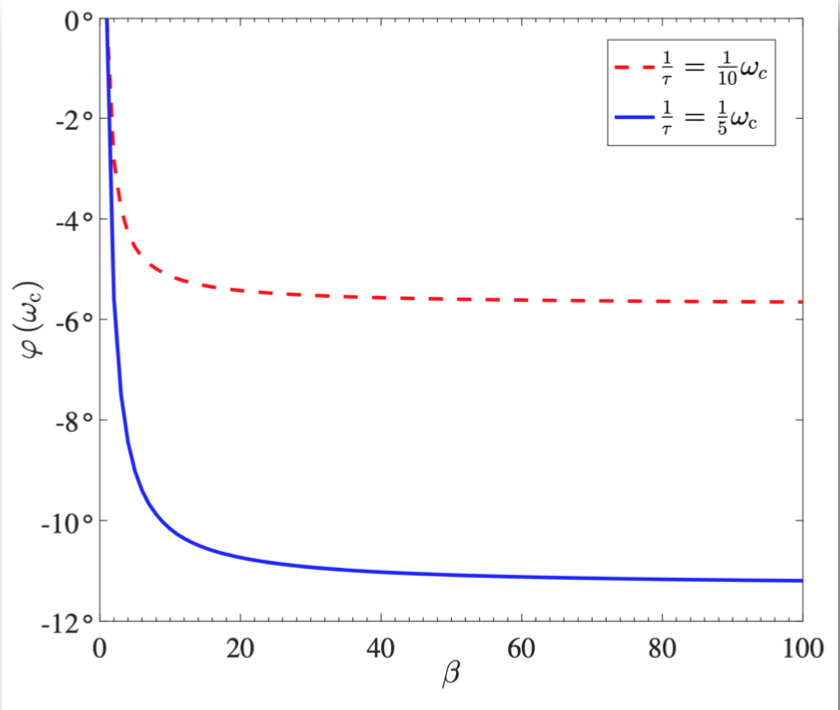
\includegraphics[width=0.7\textwidth]{./figures/lagBeta.png} 
						\caption{$\beta $ 值和迟后相角的关系}
						\label{fig:lagBeta}
					\end{figure}
			\end{itemize}  

			\subsubsection{迟后校正设计}%
			\label{ssub:迟后校正设计}
			
				\begin{enumerate}[\textbf{Step} 1.]
					\item 按稳态性能指标确定型别$\nu$ 和开环增益$K$. 
					\item 求取未校正系统$\omega_0$, $\gamma_0$, $L_{g 0}$. 
					\item 根据要求确定校正后系统的剪切频率$\omega_c$. 
						\begin{itemize}%[$\triangleright$]
							\item 满足剪切频率要求:
								\[
								\omega_c > \omega_{cL}
								.\] 
							\item 满足相位裕度要求:
								\[
									\gamma_0(\omega_c) \ge \gamma + \Delta
								,\] 
								其中$\Delta $ 为迟后环节带来的相差,取$6^\circ \sim 12^\circ$. (该处相差选择与迟后环节的$\tau$ 值选择相关,具体关系见\ref{ssub:迟后校正环节}) 
						\end{itemize}  
					\item 确定$\beta $. 使校正后系统在设计剪切频率$\omega_c$ 处幅值为0dB:
						\[
							20\lg \left| G_0(\mathrm{j} \omega_c) \right| = 20\lg \beta  
						,\] 
						即 
						\[
						\beta = \left| G_0(\mathrm{j} \omega_c) \right|
						.\] 
					\item 确定迟后环节。选择$\tau$值: 
						\[
							\dfrac{1}{\tau} = \left( \dfrac{1}{5} \sim \dfrac{1}{10} \right) \omega_c	
						,\] 
						\[
						T = \beta \tau
						.\] 
						(转折频率离剪切频率越远,带来的相差越小)。 
					\item 校验。
				\end{enumerate} 


		\subsection{串联迟后 -- 超前校正}%
		\label{sub:串联迟后_超前校正}
		
			\begin{itemize}
				\item 对于大多数系统,校正前的剪切频率已经大于要求的剪切频率,但相角不满足要求,而且要求的剪切频率处的相角储备也远小于相位裕度要求,故仅单一使用串联迟后或串联超前校正都不能达到目的,此时就需要使用串联迟后 -- 超前校正。
			\end{itemize}  

			\subsubsection{迟后环节优先的迟后-超前校正设计}%
			\label{ssub:迟后环节优先的迟后_超前校正设计}
			
				\begin{enumerate}[\textbf{Step} 1.]
					\item 确定型别与开环增益。
					\item 迟后校正。
						\begin{itemize}
							\item 考虑到后面超前环节所造成的剪切频率增长,该环节所选择的期望剪切频率$\omega_{c 1}$应略低于设计要求下界(玄学估计:一般低个$1$ rad/s差不多了)。
							\item 利用\ref{ssub:迟后校正设计} 中的步骤确定迟后校正环节$G_{c 1}(s)$. 
						\end{itemize} 
					\item 超前校正。
						\begin{itemize}
							\item 选用\ref{ssub:单级超前校正设计}中的各种设计方法,在上一步的基础上进行超前校正设计,确定超前校正环节$G_{c 2}(s)$. 
						\end{itemize}  
					\item 校验。
						\begin{itemize}
							\item 若不满足要求返回 \textbf{Step} 3 进行修正。
							\item 若通过校验则可确定整个校正环节
								\[
									G_{c}(s)=G_{c 1}(s) G_{c2}(s)
								.\] 
						\end{itemize}  
				\end{enumerate} 

			\subsubsection{超前环节优先的迟后-超前校正设计1}%
			\label{ssub:超前环节优先的迟后_超前校正设计1}
			
			\begin{itemize}
				\item 迟后环节用于提高稳态精度
			\end{itemize} 

				\begin{enumerate}[\textbf{Step} 1.]
					\item 确定型别和开环增益. 
					\item 超前校正.
						\begin{enumerate}
							\item \textbf{适当} 降低开环增益至$K_1$, 使得对应剪切频率$\omega_{01}$略小于要求的剪切频率下界$\omega_{cL}$. 
							\item 确定超前相角$\varphi_{m}$ : 
								\[
									\varphi_{m} = \gamma - \gamma_{01}(\omega_{cL}) + \Delta_1 + \Delta_2
								,\] 
								其中,$\Delta_1$ 是超前环节影响剪切频率而造成的相位损失,$\Delta_2$ 为后续迟后环节造成的相位损失,二者取值各自参考超前校正设计及迟后校正设计。
							\item 确定参数$\alpha$ : 
								\[
								\alpha = \dfrac{1+\sin\varphi_{m}}{1-\sin\varphi_{m}} 
								.\] 
							\item 确定整个迟后 -- 超前校正后的剪切频率$\omega_c$ : 
								\[
									20\lg \left| G_{01}(\omega_c) \right| = -10\lg \alpha
								.\] 
								若不满足要求,则采取以下两种策略之一进行修正:
								\begin{itemize}
									\item[$\triangleright$] 回 (b) 修正(增大)$\Delta$. 
									\item[$\triangleright$] 回 (a) 适当(玄学)增大$K_1$. 
								\end{itemize} 
							\item 确定超前环节. 最优频率$\omega_{m}$对准目标剪切频率$\omega_{c}$, 求T和$\tau$:
								\[
								T = \dfrac{1}{\omega_{m}\sqrt{\alpha}}
								,\] 
								\[
								\tau = \alpha T	
								.\]
						\end{enumerate}
					\item 校验超前校正后的系统$G_1(s)$ ,注意估计其相位裕度是否足以补偿迟后环节的相位延迟。
					\item 用于提高稳态精度的迟后校正. 
						\begin{enumerate}
							\item 确定$\beta $ :
								\[
								\beta = \dfrac{K}{K_1}
								.\] 
							\item 利用\ref{ssub:迟后校正设计}中相关步骤确定迟后环节
								\[
									\beta G_2(s) = \beta \dfrac{\tau s+1}{\beta \tau s+1} 
								.\] 
						\end{enumerate} 
					\item 校验$G(s) = G_1(s)G_2(s)$ 性能指标。如不满足要求,返回\textbf{Step} 2.(a). 
				\end{enumerate} 


			\subsubsection{超前环节优先的迟后-超前校正设计2}%
			\label{ssub:超前环节优先的迟后_超前校正设计2}
			
			\begin{itemize}
				\item 迟后环节用于降低剪切频率
			\end{itemize} 

				\begin{enumerate}[\textbf{Step} 1.]
					\item 确定型别、开环增益. 并求取$\omega_{c 0}$, $\gamma_0$, $L_{g 0}$. 
					\item 超前校正:
						\begin{enumerate}
							\item 直接选取迟后 -- 超前校正后的目标剪切频率$ \omega_c$. 
							\item 由超前相角$\varphi_{m}$ 确定参数$\alpha$. 
								\[
									\varphi_{m} = \gamma - \gamma_{0}(\omega_{c}) + \Delta_1 + \Delta_2
								,\] 
								\[
								\alpha = \dfrac{1+\sin\varphi_{m}}{1-\sin\varphi_{m}} 
								.\] 
								式中各量解释参见\ref{ssub:超前环节优先的迟后_超前校正设计1}. 
							\item 确定超前环节$G_{c 1}(s)$. 令$\omega_{m}=\omega_c$:
								\[
								T = \dfrac{1}{\omega_{m}\sqrt{\alpha}}
								,\] 
								\[
								\tau = \alpha T	
								.\]
						\end{enumerate} 
					\item 迟后校正.
						\begin{enumerate}
							\item 确定$\beta $. 使超前校正后的系统$G_1(s) = G_{c 1}(s)G_0(s)$ 在目标剪切频率处$\omega_c$ 的幅值降至0dB: 
								\[
									20\lg \beta = 20\lg \left| G_1(\mathrm{j} \omega_c) \right| 
								,\] 
								即
								\[
								\beta = \left| G_1(\mathrm{j} \omega_c) \right| 
								.\] 
							\item 选取$\tau$, 确定迟后环节
								\[
									G_{c 2}(s) = \dfrac{\tau s+1}{\beta\tau s+1} 
								.\] 
						\end{enumerate} 
					\item 校验$G(s)=G_{c 1}(s)G_{c 2}(s)G_0(s)$性能指标. 如不满足要求,回\textbf{Step} 2.  

				\end{enumerate} 

		\subsection{期望频率特性法}%
		\label{sub:期望频率特性法}
		
			\subsubsection{中频段设计}%
			\label{ssub:中频段设计}
	
				中频段宽度:
				\begin{equation}
				\label{eq:midFreqWidth}
				h \triangleq \dfrac{1+\sin \gamma }{1-\sin \gamma} 
				.\end{equation}

				\begin{alg}[对称最佳法]  
				\label{alg:对称最佳法}
					\begin{equation}
					\label{eq:对称最佳}
					\begin{cases}
						\omega_2 \le  \dfrac{\omega_c }{\sqrt{h}}\\ 
						\omega_3 \ge \omega_c \sqrt{h} 
					\end{cases} 
					\end{equation} 
				\end{alg} 

				\begin{alg}[剪切频率错位法]  
				\label{alg:剪切频率错位法}
					\begin{equation}
					\label{eq:剪切频率错位}
						\begin{cases}
							\omega_2 \le \omega_c \dfrac{2}{h+1} \\ 
							\omega_3 \ge  \omega_c \dfrac{2h}{h+1} 
						\end{cases} 
					\end{equation} 	
				\end{alg} 

				\begin{alg}[最小峰值法]  
				\label{alg:最小峰值法}
					\begin{equation}
					\label{eq:最小峰值}
						\begin{cases}
							\omega_2 \le  \omega_c \dfrac{M_r -1}{M_r} \\ 
							\omega_3 \ge  \omega_c \dfrac{M_r+1}{M_r} 
						\end{cases} 
					\end{equation} 
				\end{alg} 

			\subsubsection{期望频率特性校正设计}%
			\label{ssub:期望频率特性校正设计}
	
				\begin{enumerate}[\textbf{Step} 1.] 
					\item 低频段设计。\\
						低频段由系统型别和稳态增益确定,一般和未校正系统相同:
						\[
							G_L(s) = \dfrac{K}{s^{v}}
						.\] 
					\item 中频段设计。 
						\begin{itemize}
							\item 斜率: $-20$ dB/dec. 
							\item 根据性能指标要求,确定剪切频率$\omega_c$ 、下限频率$\omega_2$ 、上限频率$\omega_3$ (可参照\ref{ssub:中频段设计})
							\item 灵活选取,尽量与未校正系统的转折频率重合,以简化控制器. 
						\end{itemize}  
					\item 中低频过渡段设计。
						\begin{itemize}
							\item 斜率:$-40$ dB/dec. 
							\item 转折频率$\omega_1$ :
								\[
									20\lg K - 20 v \lg \omega_c - 20(2-v)\lg \dfrac{\omega_c}{\omega_1} + 20 \lg \dfrac{\omega_c}{\omega_2 } = 0 
								\]
								$\implies $
								\[
								\dfrac{K \omega_1^{2-v} }{\omega_c \omega_{2}} = 1
								.\] 
						\end{itemize} 
					\item 高频段设计:等于或平行于未校正系统。
					\item 中高频过渡段设计
						\begin{itemize}
							\item 一般出于简单起见,转折频率$\omega_4$ (及$\omega_5$)选取未校正系统的转折频率. 
						\end{itemize} 
					\item 校验。
						\begin{itemize}
							\item 期望频率特性$G(s)$,检验性能指标。
							\item 如不满足,回\textbf{Step} 2. 重新设计。
						\end{itemize} 
					\item 求取校正装置传递函数:
						\[
							G_c(s) = \dfrac{G(s)}{G_0(s)}
						.\] 
				\end{enumerate} 

	\newpage 
	
	\section{根轨迹校正方法}%
	\label{sec:根轨迹校正方法}
        Credit by F. C. Zhu. 

        Start from the next page. 
        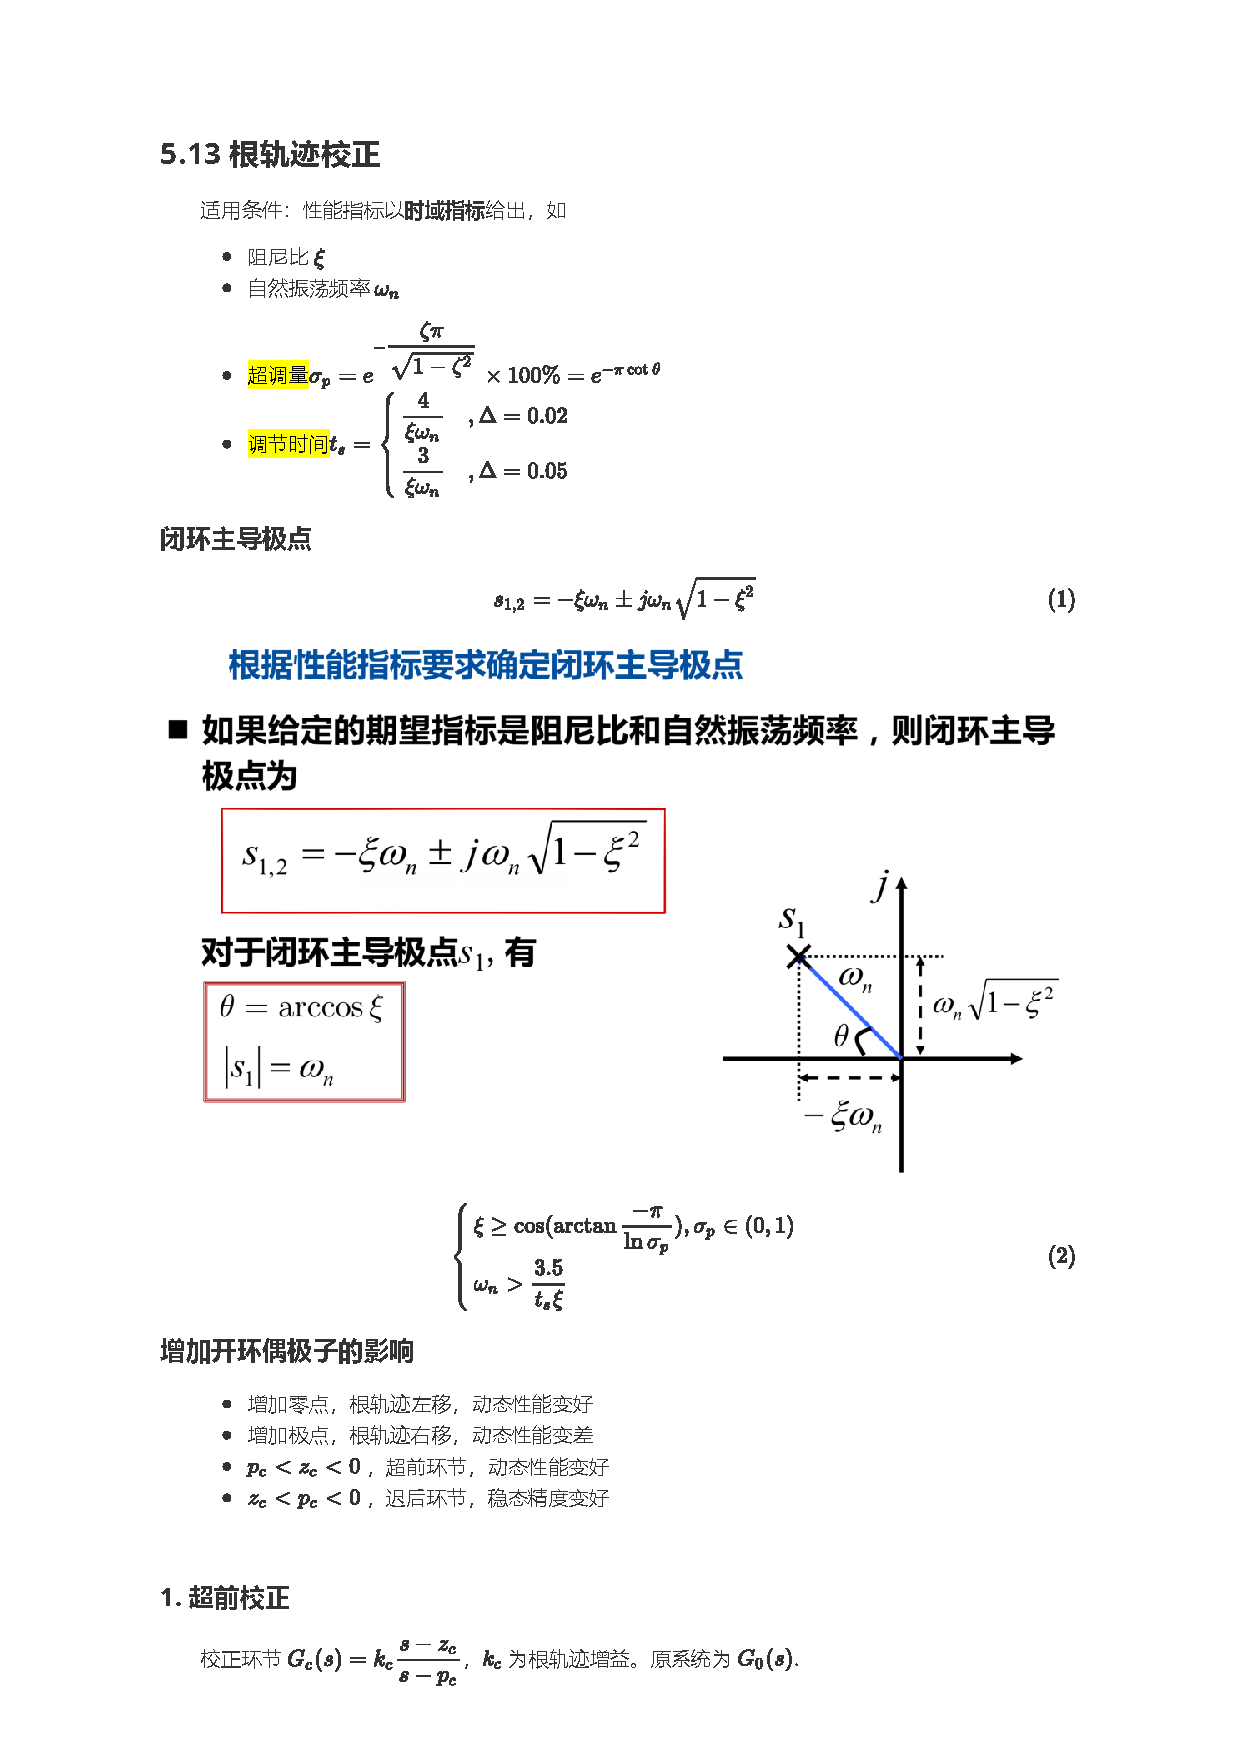
\includepdf[pages=-]{rootlocus_ZFC.pdf}

	\newpage
	\section{线性系统的能控性和能观性}%
	\label{sec:线性系统的能控性和能观性}
	
		\subsection{能控性}%
		\label{sub:能控性}
		
			\begin{dfn}[能控状态]  
			\label{dfn:能控状态}
			对于\textbf{线性定常系统} ,若对于确定初始时刻$t_0$的状态$\overline{x}$ ,$\exists t_1>0$ 和一个无约束的容许控制$u(t),\ t\in\left[ t_0,t_1 \right]$ ,使得系统在该作用下,系统状态经过时间$t_1-t_0$ 后转移到$x(t_1)=0$,则称$\overline{x}$是系统在$t_0$ 时刻的一个能控状态。
			\end{dfn} 

			\begin{dfn}[能达状态]  
			\label{dfn:能达状态}
			对于\textbf{线性定常系统} ,若对于确定初始时刻$t_0$的状态$x(t_0)=0$ ,$\exists t_1>0$ 和一个无约束的容许控制$u(t),\ t\in\left[ t_0,t_1 \right]$ ,使得系统在该作用下,系统状态经过时间$t_1-t_0$ 后转移到$x(t_1)=\overline{x}$,则称$\overline{x}$是系统在$t_0$ 时刻的一个能达状态。
			\end{dfn} 

			现有线性定常系统
			\begin{equation}
			\label{eq:LTI}
			\begin{cases}
				\begin{aligned}
					\dot x(t) &= Ax(t) + Bu(t) \\ 
					y(t) &= Cx(t)
				\end{aligned}  
			\end{cases} 
			.\end{equation} 

			\begin{dfn}[能控性]  
			\label{dfn:能控性}
				对于线性定常系统\eqref{eq:LTI},如果状态空间中所有非零状态都是能控的,则称系统\eqref{eq:LTI}是能控的。	
			\end{dfn} 

			\begin{dfn}[能达性]  
			\label{dfn:能达性}
				对于线性定常系统\eqref{eq:LTI},如果状态空间中所有非零状态都是能达的,则称系统\eqref{eq:LTI}是能达的。	
			\end{dfn} 

			\begin{rmk}[连续定常系统的能控性与能达性关系]  
			\label{rmk:能控性与能达性关系}
				对于\textbf{连续线性定常}系统,能控性$\Leftrightarrow$能达性。
			\end{rmk} 

			\subsubsection{能控性判据}%
			\label{ssub:能控性判据}
			
				\begin{thm}[Gram矩阵判据]  
				\label{the:gram矩阵判据}
					连续\textbf{线性定常}系统完全可控的\emph{充要条件}是,存在时刻$t_1>0$,使得Gram矩阵
					\begin{equation}
					\label{eq:gram}
					W_c(0,t_1) = \int_0^{t_1} e^{-At}BB^{\text{T}}e^{-A^{T}t}\ \mathrm{d}t	
					\end{equation} 
					为非奇异的。
				\end{thm}

				\begin{nnt} 
					线性定常系统是能打的,当且仅当存在时刻$t_1>0$ ,使得Gram矩阵\eqref{eq:gram}非奇异。
				\end{nnt} 

				\begin{nnr}  
					对于连续线性定常系统,从证明过程可看出,以上两定理中的表述$\exists t_1$ 表述可改为更为严格的条件:$\forall t_1>0$. 
				\end{nnr} 


				\begin{thm}[能控矩阵判据]  
				\label{the:能控矩阵判据}
					连续线性定常系统完全可控的\emph{充要条件}是
					\begin{equation}
					\label{eq:Qc}
						\mathop{\textnormal{rank}} Q_c = \mathop{\textnormal{rank}} \begin{bmatrix}
							B & AB & \cdots & A^{n-1}B
						\end{bmatrix} = n
					.\end{equation}
					其中,
					\[
					n \triangleq \mathop{\textnormal{rank}} A 
					,\] 
					\[
					Q_c \triangleq 
						 \begin{bmatrix}
							B & AB & \cdots & A^{n-1}B
						\end{bmatrix} 
					.\] 
				\end{thm} 

				\begin{thm}[PBH秩判据]  
				\label{the:pbh秩判据}
				线性定常系统\eqref{eq:LTI}能控的\emph{充分必要}条件是系统矩阵$A$ 的所有特征值满足
				\begin{equation}
				\label{eq:PBH}
					\mathop{\textnormal{rank}} \begin{bmatrix}
						\lambda_{i}I - A & B 
					\end{bmatrix} = n \ ,\quad i=1,\ldots n
				\end{equation} 
				或可以等价地表示为
				\begin{equation}
				\label{eq:PBH_2}
					\mathop{\textnormal{rank}} \begin{bmatrix}
						sI - A & B 
					\end{bmatrix} = n \ , \quad \forall s\in \mathbb{C}
				.\end{equation}		
				\end{thm} 

				\begin{thm}[Jordan标准型判据]  
				\label{the:jordan标准型判据}
					LTI连续系统能控的\emph{充分必要}条件分两种情况。
					\begin{enumerate}[(1)]
						\item 状态矩阵$A$ 的特征值各不相同时,导出的对角规范型为
							\[
								\dot{ \overline{x}} = \begin{bmatrix}
								\lambda_1 & & & 0\\
										  & \lambda_2 & &\\
								&&\ddots &\\
								0 &&& \lambda_{n}
							\end{bmatrix} \overline{x} + \overline{B} \overline{u}
							\]
							则系统能控的充要条件是 $\overline{B}$ 不包含元素全为零的行。
						\item 状态矩阵有重特征值时,矩阵$A$ 写成Jordan标准型,并将输入矩阵写成相应的分块形式
							\[
							A = \begin{bmatrix}
								J_{11} &&&&&&&&&0 \\
									   & J_{12} &&&&&&&&\\
									   &&\ddots &&&&&&&\\
									   &&&J_{1 q_1} &&&&&&\\
									   &&&&J_{21}&&&&&\\
									   &&&&&\ddots &&&&\\
									   &&&&&&J_{l 1}&&&\\
									   &&&&&&&J_{l 2}&&\\
									   &&&&&&&&\ddots & \\
										0&&&&&&&&&J_{l q_l}
							\end{bmatrix} 
							,\] 
							\[
							B = \begin{bmatrix}
								b_{11}\\
								b_{12}\\
								\vdots\\
								b_{1q_1}\\
								b_{21}\\
								\vdots\\
								b_{l 1}\\
								b_{l 2}\\ 
								\vdots\\
								b_{lq_l}
							\end{bmatrix} 
							\]
							其中,$q_{i}$ 是特征值$\lambda_{i}$ 对应的几何重数(特征值$\lambda_{i}$所包含的Jordan小块的个数)。\\
							则,系统能观的充要条件是 分块矩阵$b_{i 1}, \cdots ,b_{iq_{i}}$ 的最后一行构成的行向量组线性无关($\forall i=1,\ldots ,l$). 
					\end{enumerate}
				\end{thm} 

				\begin{cor}  
					若\textbf{单输入系统} 具有重特征值,则系统不能控。
				\end{cor} 

				\begin{prop}  
				\label{prop:能控性在非奇异线性线性变换下的属性}
					对于线性定常系统$\left( A,B,C \right)$,经线性非奇异变换为$\left( \overline{A},\overline{B},\overline{C} \right)$ ,二者之间有如下关系:
					\[
					\overline{A}=PAP^{-1}
					,\] 
					\[
					\overline{B} = PB
					,\] 
					\[
					\overline{C} = CP^{-1}
					,\]
					\[
					\mathop{\textnormal{rank}} Q_c = \mathop{\textnormal{rank}} \overline{Q}_c
					.\] 
				\end{prop} 


		\subsection{能观性}%
		\label{sub:能观性}
		
			已知系统输入和输出,能否决定状态? \\ 
			现有系统
			\begin{equation}
			\label{eq:freeSys}
				\begin{cases}
					\begin{aligned}
						\dot x &= A(t)x\ , \quad x(t_0) = x_0 \ , \quad t\ge t_0 \\ 
						y &= C(t)x
					\end{aligned}  
				\end{cases} 
			\end{equation} 
		
			\begin{dfn}[能观状态]  
			\label{dfn:能观状态}
			对于线性系统\eqref{eq:freeSys},如果对于初始时刻$t_0$ 的一个非零初始状态$x_0$ ,存在一个有限时刻$t_1>t_0$,使得区间$[t_0, t_1]$ 上的系统输出$y(t)$ 可以唯一决定系统的初始状态$x_0$ ,则称状态$x_0$ 在时刻$t_0$ 为能观测的。				
			\end{dfn} 

			\begin{dfn}[系统能观性]  
			\label{dfn:系统能观性}
				若对于状态空间中的所有状态$x_0$ 都是在时刻$t_0$ 能观的,则称系统在时刻$t_0$ 是完全能观的。若$\forall t_0\in [T_1,T_2]$ ,系统均是在$t_0$ 时刻能观的,则称系统在区间$[T_1, T_2]$ 上是完全能观的。	
			\end{dfn} 

			\subsubsection{能观性判据}%
			\label{ssub:能观性判据}
			
				现有线性定常连续系统
				\begin{equation}
				\label{eq:LTIF}
					\begin{cases}
						\begin{aligned}
							\dot x &= Ax \ ,\quad x(0)=x_0\ ,\quad t\ge 0 \\ 
							y &= Cx
						\end{aligned}  
					\end{cases} 
				\end{equation} 

				\begin{thm}[能观性Gram矩阵判据]  
				\label{the:能观性gram矩阵判据}
					线性定常连续系统\eqref{eq:LTIF}能观的充分必要条件是存在有限时刻$t_1>0$ ,使Gram矩阵
					\begin{equation}
					\label{eq:gram_ob}
					W_o(0,t_1) \triangleq \int_0^{t_1} e^{A^Tt}C^T C e^{At}\ \mathrm dt
					\end{equation} 
					非奇异。
				\end{thm} 

				\begin{thm}[能观性矩阵判据]  
				\label{the:能观性矩阵判据}
					LTI系统\eqref{eq:LTIF}能观的\emph{充分必要条件}是
					\[
					\mathop{\textnormal{rank}} Q_o = n 
					,\] 
					其中
					\[
						Q_o \triangleq \begin{bmatrix}
							C \\ 
							CA \\
							\vdots\\
							CA^{n-1}
						\end{bmatrix} 
					.\] 
				\end{thm} 

				\begin{thm}[]  
				\label{the:}
				LTI连续系统\eqref{eq:LTIF}完全能观的\emph{充分必要}条件是,$A$ 没有与$C$ 的所有行都正交的非零右特征向量,i.e.  
				\[
					\forall \ \lambda_{i},\ \textnormal{s.t. } 
					\begin{cases}
						A\alpha = \lambda_{i}\alpha \\
						C \alpha = 0
					\end{cases}
					\implies \quad \alpha \equiv 0
				.\] 
				\end{thm} 

				\begin{thm}[能观性Jordan标准型判据]  
				\label{the:能观性jordan标准型判据}
					LTI连续系统能观的\emph{充分必要}条件分两种情况。
					\begin{enumerate}[(1)]
						\item 状态矩阵$A$ 的特征值各不相同时,导出的对角规范型为
							\[
								\begin{split}
									\dot{ \overline{x}} &= \begin{bmatrix}
								\lambda_1 & & & 0\\
										  & \lambda_2 & &\\
								&&\ddots &\\
								0 &&& \lambda_{n}
								\end{bmatrix} \overline{x} \\ 
										y &= \overline{C} \overline{x}
								\end{split}
							\]
							则系统能观的充要条件是 $\overline{C}$ 不包含元素全为零的列。
						\item 状态矩阵有重特征值时,矩阵$A$ 写成Jordan标准型,并将输入矩阵写成相应的分块形式
							\[
							A = \begin{bmatrix}
								J_{11} &&&&&&&&&0 \\
									   & J_{12} &&&&&&&&\\
									   &&\ddots &&&&&&&\\
									   &&&J_{1 q_1} &&&&&&\\
									   &&&&J_{21}&&&&&\\
									   &&&&&\ddots &&&&\\
									   &&&&&&J_{l 1}&&&\\
									   &&&&&&&J_{l 2}&&\\
									   &&&&&&&&\ddots & \\
										0&&&&&&&&&J_{l q_l}
							\end{bmatrix} 
							,\] 
							\[
								C = \begin{bmatrix}
									c_{11} & c_{12} & \cdots  & c_{1 q_1} & c_{21} & \cdots & c_{l 1} & c_{l 2} & \cdots  & c_{l q_l} 
								\end{bmatrix} 
							\]
							其中,$q_{i}$ 是特征值$\lambda_{i}$ 对应的几何重数。\\
							则,系统能观的充要条件是:分块矩阵$c_{i 1}, \cdots ,c_{iq_{i}}$ 的第一列线性无关($\forall i=1,\ldots ,l$). 
					\end{enumerate}
				\end{thm} 
			\subsubsection{对偶原理}%
			\label{ssub:对偶原理} 

				\begin{dfn}[对偶系统]  
				\label{dfn:对偶系统}
					线性系统
					\[
					\begin{cases}
						\dot x = Ax \\ 
						y = Cx
					\end{cases} 
					\] 
					与
					\[
					\dot z = A^{\textnormal{T}} z + C^{\textnormal{T}} v
					\]
					互为对偶系统;同理,系统
					\[
					\begin{cases}
						\dot x = Ax + Bu
					\end{cases} 
					\] 
					与
					\[
						\begin{cases}
							\dot z = A^{\textnormal{T}} z \\
							w = B^{\textnormal{T}} z
						\end{cases} 
					\]
					互为对偶系统。
				\end{dfn}  

				\begin{thm}[对偶原理]  
				\label{the:对偶原理}
					线性系统$\Sigma$ 的能控性和能观性,分别与其对偶系统$\Sigma^*$ 的能观性和能控性等价。
				\end{thm} 

		\subsection{连续系统的结构分解}%
		\label{sub:连续系统的结构分解}

			现有一能控的SISO线性定常系统
			\begin{equation}
			\label{eq:siso_lti}
				\begin{cases}
					\begin{aligned}
						\dot x &= Ax + bu \\ 
						y &= cx
					\end{aligned}  
				\end{cases} 
			\end{equation} 
			且系统特征多项式为
			\begin{equation}
			\label{eq:siso_lti_cp}
			\alpha(s) = s^{n} + \alpha_{n-1}s^{n-1}+ \cdots  + \alpha_1 s + \alpha_0	
			.\end{equation} 
		
			\subsubsection{规范型}%
			\label{ssub:规范型}
			
				\begin{thm}[第一能控规范型]  
				\label{the:第一能控规范型}
					引入非奇异线性变换
					\[
					\overline{x} = Px,\quad P = Q_c^{-1}
					,\] 
					即可导出系统\eqref{eq:siso_lti}第一能控规范型
					\begin{equation}
					\label{eq:ctrl_canonical}
						\begin{cases}
							\begin{aligned}
								\dot{\overline{x}} &= A_c \overline{x} + b_c u \\
								y &= c_c \overline{x}
							\end{aligned}  
						\end{cases} 
					,\end{equation}
					其中,
					\begin{equation}
					\label{eq:ctrl_canonical_1_Ab}
						A_c = \begin{bmatrix}
							0 & \cdots & 0& -\alpha_0 \\ 
							1 & \cdots & 0&-\alpha_1 \\ 
							\vdots &&\vdots&\vdots \\ 
							0 & \cdots & 1 & -\alpha_{n-1}
						\end{bmatrix} \quad 
						b_c = \begin{bmatrix}
							1 \\ 
							0 \\ 
							\vdots\\
							0
						\end{bmatrix} 
					\end{equation} 
					\begin{equation}
					\label{eq:ctrl_canonical_1_c}
					\begin{aligned}
						c_c = cQ_c = \begin{bmatrix}
							\beta_0 & \beta_1 & \cdots & \beta_{n-1}
						\end{bmatrix},\\ 
						\quad \beta_{i}=cA^i b,\quad i=0,1,\ldots ,n-1.
					\end{aligned}  
					\end{equation} 
				\end{thm} 

				\begin{thm}[第二能控规范型]  
				\label{the:第二能控规范型} 
					定义变换矩阵$P$ 
					\[
					P \triangleq Q_c H_A = \begin{bmatrix}
						b & Ab & \cdots & A^{n-1}b 
					\end{bmatrix} \begin{bmatrix} 
						\alpha_1 & \alpha_2 & \cdots  & \alpha_{n-1} & 1 \\
						\alpha_2 & \alpha_3 & \cdots & 1 \\
						\vdots & & \iddots \\
						\alpha_{n-1} & \iddots \\
						1
					\end{bmatrix} 
					,\]
					则,通过非奇异线性变换$\overline{x}=P^{-1}x$ 可将系统\eqref{eq:siso_lti}转化为第二能控规范型\eqref{eq:ctrl_canonical},其中
					\begin{equation}
					\label{eq:ctrl_canonical_2_Ab}
						A_c = \begin{bmatrix}
							0 & 1& \cdots & 0\\ 
							\vdots &\vdots&\ddots&\vdots \\ 
							0 & 0& \cdots &1 \\ 
							-\alpha_0 & -\alpha_1 & \cdots  & -\alpha_{n-1}
						\end{bmatrix} \quad 
						b_c = \begin{bmatrix}
							0 \\ 
							0 \\ 
							\vdots\\
							1
						\end{bmatrix} 
					\end{equation} 
					\begin{equation}
					\label{eq:ctrl_canonical_2_c}
					\begin{aligned}
						c_c = cP = \begin{bmatrix}
							\beta_0 & \beta_1 & \cdots & \beta_{n-1}
						\end{bmatrix},\\ 
						\begin{cases}
							\beta_{n-1} = c b \\ 
							\beta_{n-2} = cAb + \alpha_{n-1}c b\\
							\vdots \\ 
							\beta_1 = cA^{n-2}b + \alpha_{n-1}cA^{n-3}b + \cdots +\alpha_2c b\\
							\beta_0 = cA^{n-1}b + \alpha_{n-1}cA^{n-2}b + \cdots +\alpha_1 c b\\
						\end{cases}. 
					\end{aligned}  
					\end{equation} 
					且系统的传递函数为
					\[
						W(s) = c_c(sI-A_c)^{-1}b_c = \dfrac{\beta_{n-1}s^{n-1}+\beta_{n-2}s^{n-2}+ \cdots +\beta_0}{s^{n}+\alpha_{n-1}s^{n-1}+\cdots +\alpha_0} 
					.\] 
				\end{thm} 

				\begin{thm}[第一能观规范型]  
				\label{the:第一能观规范型}
				假设系统\eqref{eq:siso_lti}完全能观,引入如下非奇异线性变换
				\[
					\tilde x = Q_o x
				,\] 
				则可导出如下第一能观规范型
				\begin{equation}
				\label{eq:obsv_canonical_1}
					\begin{split}
						\dot{\tilde x} &= \begin{bmatrix}
							0 & 1& \cdots & 0\\ 
							\vdots &\vdots&\ddots&\vdots \\ 
							0 & 0& \cdots &1 \\ 
							-\alpha_0 & -\alpha_1 & \cdots  & -\alpha_{n-1}
					\end{bmatrix} \tilde x + \begin{bmatrix}
						\beta_0\\
						\beta_1\\
						\vdots\\
						\beta_{n-1}
					\end{bmatrix} u \\ 
					y &= \begin{bmatrix}
						1 & 0 & \cdots & 0 
					\end{bmatrix} \tilde x
					\end{split}
				\end{equation}
				其中$\beta $ 由式\eqref{eq:ctrl_canonical_1_c}给出。
				\end{thm} 

				\begin{thm}[第二能观规范型]  
				\label{the:第二能观规范型}
				假设系统\eqref{eq:siso_lti}完全能观,引入如下非奇异线性变换
				\[
					\tilde x = Q x, \quad Q \triangleq H_A Q_o
				,\] 
				则可导出如下第二能观规范型
				\begin{equation}
				\label{eq:obsv_canonical_2}
					\begin{split}
						\dot{\tilde x} &= \begin{bmatrix}
							0 & 1& \cdots & 0\\ 
							\vdots &\vdots&\ddots&\vdots \\ 
							0 & 0& \cdots &1 \\ 
							-\alpha_0 & -\alpha_1 & \cdots  & -\alpha_{n-1}
					\end{bmatrix} \tilde x + \begin{bmatrix}
						\beta_0\\
						\beta_1\\
						\vdots\\
						\beta_{n-1}	
					\end{bmatrix} u \\ 
					y &= \begin{bmatrix}
						0& 0 & \cdots & 1 
					\end{bmatrix} \tilde x
					\end{split}
				\end{equation}
				其中$\beta $ 由式\eqref{eq:ctrl_canonical_2_c}给出。
				\end{thm} 
			
			\subsubsection{能控性结构分解}%
			\label{ssub:能控性结构分解}
			
				\begin{alg}[能控性结构分解的求取]  
				\label{alg:能控性结构分解的求取}
					\ 
					\begin{enumerate}[\textbf{Step} 1.]
						\item 列写能控性矩阵 
							\[
							Q_c = \begin{bmatrix}
								B & AB & \cdots & A^{n-1}B 
							\end{bmatrix} 
							,\] 
							并求$\mathop{\textnormal{rank}} Q_c = k$. 
						\item 从$Q_c$ 中选取$k$ 个线性无关的列向量$q_1,\ldots ,q_{k}$ ,再从$\mathbb{R}^{n}$ 中任选$n-k$ 个列向量$q_{k+1},\ldots ,q_{n}$ ,使向量组 $\left\{ q_1,\ldots q_{k},q_{k+1},\ldots ,q_{n} \right\}$ 线性无关。 
						\item 构造变换阵
							\[
							P^{-1} \triangleq \begin{bmatrix}
								q_1 & \cdots &q_{k} & q_{k+1} & \cdots & q_{n} 
							\end{bmatrix} 
							.\] 
						\item 系统变换
							\[
							\overline{x}=Px,\quad\overline{A}=PA P^{-1},\quad \overline{B}=PB,\quad \overline{C}=CP^{-1}
							,\] 
							变换后系统为
							\[
							\begin{cases}
								\dot{\overline{x}} = \overline{A} \overline{x} + \overline{B} u \\ 
								y = \overline{C} x
							\end{cases} 
							.\] 
					\end{enumerate} 
				\end{alg} 

				\begin{rmk}[算法说明]  
				\label{rmk:算法说明}
					上述算法中,若能控性矩阵较大,则欲找出$Q_c$ 的极大无关组并不容易。实际上,从证明过程中可看出,只需要找出$Q_c$ 的列向量空间的一组基即可。
				\end{rmk} 
			
				\begin{thm}[能控性结构分解]  
				\label{the:能控性结构分解}
				对于MIMO不完全能控LTI系统\eqref{eq:LTI},利用Algorithm \ref{alg:能控性结构分解的求取},则系统可化为能控性分解的规范形式
				\begin{equation}
				\label{eq:ctrl_decmp}
					\begin{cases}
						\begin{aligned}
							\begin{bmatrix}
								\dot{\overline{x}}_c\\
								\dot{\overline{x}}_{\bar c}\\
							\end{bmatrix} &= \begin{bmatrix}
							\overline{A}_c & \overline{A}_{12} \\ 
							0 & \overline{A}_{\overline{c}}
							\end{bmatrix}  
							\begin{bmatrix}
								{\overline{x}}_c\\
								{\overline{x}}_{\bar c}\\
							\end{bmatrix} + \begin{bmatrix}
								\overline{B}_c \\
								0
							\end{bmatrix} u \\ 
							y &= \begin{bmatrix}
								\overline{C}_c & \overline{C}_{\overline{c}} 
							\end{bmatrix} 
							\begin{bmatrix}
								{\overline{x}}_c\\
								{\overline{x}}_{\bar c}\\
							\end{bmatrix} 
						\end{aligned}  
					\end{cases} 
				.\end{equation}
				并且有如下结论 
				\begin{enumerate}[(1)]
					\item 系统$\left( \overline{A}_c, \overline{B}_c \right) $ 完全能控;
					\item 子系统$\left( \overline{A}_c, \overline{B}_c, \overline{C}_c \right)$ 的传递函数等于整个系统的传递函数,i.e. 
						\[
							\overline{C}_c \left( sI - \overline{A}_c \right)^{-1} \overline{B}_c = C(sI-A)^{-1}B
						.\] 
				\end{enumerate} 
				\end{thm} 

				\begin{rmk}[能控结构分解]  
				\label{rmk:能控结构分解}
					从上述定理可看出,能控性分解将系统分解为完全能控和完全不能控的两个子系统。其中$k$ 维能控子系统为
					\[
					\begin{cases}
						\dot{\overline{x}}_c = \overline{A}_c \overline{x}_c + \overline{A}_{12} \overline{x}_{\overline{c}} + \overline{B}_c u \\ 
						y_1 = \overline{C}_c \overline{x}_c
					\end{cases} 
					\]
					不能控$n-k$ 维子系统为
					\[
					\begin{cases}
						\dot{\overline{x}}_{\overline{c}} = \overline{A}_{\overline{c}} \overline{x}_{\overline{c}} \\ 
						y_2 = \overline{C}_{\overline{c}} \overline{x}_{\overline{c}}
					\end{cases} 
					.\] 
				\end{rmk} 
				\begin{rmk}[能控振型]  
				\label{rmk:能控振型}
					由上述定理知:
					\[ 
						\begin{split}
							\mathop{\text{det}} (sI-A)
							&= \mathop{\text{det}} (sI-\overline{A} )\\
							&= \mathop{\text{det}} \begin{bmatrix}
								sI - \overline{A}_c & -\overline{A}_{12}\\
								0 & sI-\overline{A}_{\overline{c}} 
							\end{bmatrix} \\
							&= \mathop{\text{det}} (sI - \overline{A}_c) \mathop{\text{det}} (sI-\overline{A}_{\overline{c}}). 
						\end{split}
					\]
					上式表明,不完全能控系统的特征值有两部分组成:一部分为$\overline{A}_c$ 的特征值,称为\emph{能控振型};另一部分为$\overline{A}_{\overline{c}}$ 的特征值,称为\emph{不能控振型}. 外部输入$u$ 只能改变能控振型的位置,无法改变不能控振型的位置. 
				\end{rmk} 

			\subsubsection{能观性结构分解}%
			\label{ssub:能观性结构分解}
			
				由对偶原理,可得如下算法与定理:

				\begin{alg}[能观性结构分解的求取]  
				\label{alg:能观性结构分解的求取}
					\ 
					\begin{enumerate}[\textbf{Step} 1.]
						\item 列写能观性矩阵
							\[
							Q_o = \begin{bmatrix}
								C\\ 
								CA\\
								\vdots\\
								CA^{n-1}
							\end{bmatrix} 
							,\] 
							并求 $\mathop{\textnormal{rank}} Q_o = k$. 
						\item 从$Q_o$ 中选取$k$ 个线性无关的行向量$q_1^T,\ldots ,q_{k}^T$ ,再从$\mathbb{R}^{n}$ 中任选$n-k$ 个行向量$q_{k+1}^T,\ldots ,q_{n}^T$ ,使向量组 $\left\{ q_1^T,\ldots q_{k}^T,q_{k+1}^T,\ldots ,q_{n}^T \right\}$ 线性无关。 
						\item 构造变换阵
							\[
							P^{-1} \triangleq \begin{bmatrix}
								q_1^T \\ \vdots \\q_{k}^T \\ q_{k+1}^T  \\ \vdots \\ q_{n}^T
							\end{bmatrix} 
							.\] 
						\item 系统变换
							\[
							\overline{x}=Px,\quad\overline{A}=PA P^{-1},\quad \overline{B}=PB,\quad \overline{C}=CP^{-1}
							,\] 
							变换后系统为
							\[
							\begin{cases}
								\dot{\overline{x}} = \overline{A} \overline{x} + \overline{B} u \\ 
								y = \overline{C} x
							\end{cases} 
							.\] 
					\end{enumerate} 
				\end{alg} 

				\begin{thm}  
				\label{the:882}
				对于MIMO不完全能观LTI系统\eqref{eq:LTI},利用Algorithm \ref{alg:能观性结构分解的求取},可得如下能观性分解的规范型:
				\begin{equation}
				\label{eq:obsv_decmp}
					\begin{cases}
						\begin{aligned}
							\begin{bmatrix}
								\dot{\overline{x}}_o\\
								\dot{\overline{x}}_{\bar o}\\
							\end{bmatrix} &= \begin{bmatrix}
							\overline{A}_o & 0\\ 
							\overline{A}_{21} & \overline{A}_{\overline{o}}
							\end{bmatrix}  
							\begin{bmatrix}
								{\overline{x}}_o\\
								{\overline{x}}_{\bar o}\\
							\end{bmatrix} + \begin{bmatrix}
								\overline{B}_o \\
								\overline{B}_{\overline{o}}	
							\end{bmatrix} u \\ 
							y &= \begin{bmatrix}
								\overline{C}_o & 0 
							\end{bmatrix} 
							\begin{bmatrix}
								{\overline{x}}_o\\
								{\overline{x}}_{\bar o}\\
							\end{bmatrix} 
						\end{aligned}  
					\end{cases} 
				.\end{equation}
				并且有如下结论 
				\begin{enumerate}[(1)]
					\item 系统$\left( \overline{A}_o, \overline{C}_o \right) $ 完全能观;
					\item 子系统$\left( \overline{A}_o, \overline{B}_o, \overline{C}_o \right)$ 的传递函数等于整个系统的传递函数,i.e. 
						\[
							\overline{C}_o \left( sI - \overline{A}_o \right)^{-1} \overline{B}_o = C(sI-A)^{-1}B
						.\] 
				\end{enumerate} 
				\end{thm}

			\subsubsection{LTI系统的规范分解}%
			\label{ssub:lti系统的规范分解}
			
				\begin{thm}[规范分解定理]  
				\label{the:规范分解定理}
				\ \\
				对于不完全能控和不完全能观的LTI系统\eqref{eq:LTI},通过非奇异线性变换可实现系统结构的规范分解。其规范分解后的表达式为
				\begin{equation}
				\label{eq:canonical_decmp}
				\begin{aligned}
					\begin{bmatrix}
						\dot x_{co} \\ 
						\dot x_{c\overline{o}}\\
						\dot x_{\overline{c}o}\\
						\dot x_{\overline{c}\overline{o}}
					\end{bmatrix} &= \begin{bmatrix}
					\tilde A_{co} & 0 & \tilde A_{13} & 0\\ 
					\tilde A_{21} & \tilde A_{c\overline{o}} & \tilde A_{23} & \tilde A_{24} \\ 
					0 & 0& \tilde A_{\overline{c}o} & 0\\ 
					0 & 0& \tilde A_{43} & \tilde A_{\overline{c}\overline{o}}
					\end{bmatrix} \begin{bmatrix}
						 x_{co} \\ 
						 x_{c\overline{o}}\\
						 x_{\overline{c}o}\\
						 x_{\overline{c}\overline{o}}
					\end{bmatrix} + \begin{bmatrix}
						\tilde B_{co} \\ 0 \\ 0\\ 0 
					\end{bmatrix} u \\
					y&= \begin{bmatrix}
						\tilde C_{co} & 0 & \tilde C_{\overline{c}o} & 0 
					\end{bmatrix} x
				\end{aligned}  
				\end{equation} 
				系统传递函数与系统的既能控又能观部分的传递函数一致,i.e. 
				\[
					G(s) = \tilde C_{co}\left( sI - \tilde A_{co} \right) ^{-1} \tilde B_{co}
				.\] 
				\end{thm} 

			\subsubsection{LTI系统由Jordan标准型的结构分解}%
			\label{ssub:lti系统由jordan标准型的结构分解}
				见书P497$\sim$P498。大致思路:将得到的Jordan标准型各状态及对应矩阵的行、列按四种情况重新排列,得到基于Jordan标准型的规范结构分解。	
			
		\subsection{状态空间实现}%
		\label{sub:状态空间实现} 

			\begin{dfn}[状态空间实现]  
			\label{dfn:状态空间实现}
			一致系统传递函数矩阵$G(s)$ ,寻找一个状态空间描述$\Sigma\left( A,B,C,D \right) $ ,满足
			\[
				G(s) = C\left( sI - A \right) ^{-1}B + D
			,\] 
			则$\Sigma\left( A,B,C,D \right) $ 为$G(s)$ 的一个状态空间实现,简称实现。矩阵$A$ 的阶数称为$G(s)$ 的实现的阶数。
			\end{dfn}

			\begin{rmk}[物理可实现条件]  
			\label{rmk:物理可实现条件}
				\ 
				\begin{enumerate}
					\item 传递函数矩阵$G(s)$ 中的每一个元$G_{ij}(s)$ 的分子分母多项式的系数均为实常数;
					\item $G(s)$ 的元$G_{ij}(s)$ 是$s$ 的真有理分式函数。
						\begin{itemize}
							\item[$\triangleright$] 若$G(s)$ 所有元素均为严格真有理分式,则实现$\Sigma $ 具有$\left( A,B,C \right)$ 的形式;
							\item[$\triangleright$] 若$G(s)$ 元素中存在相对阶为0的传递函数,则实现$\Sigma $ 具有\\$\left( A,B,C,D \right)$ 的形式,且
								\[
									\lim_{s\to \infty}G(s) = \lim_{s\to \infty} \left[ C(sI-A)^{-1}B+D \right] = D
								.\] 
						\end{itemize}  
				\end{enumerate} 
			\end{rmk} 

			\begin{thm}[ ]  
			\label{the:821}
				对于SISO系统,一个传递函数的实现是能控能观的\emph{充要条件}是传递函数无零极点对消。
			\end{thm} 

			\subsubsection{SISO系统的实现}%
			\label{ssub:siso系统的实现}
		
				见``自控理论A''中``传递函数导出状态空间模型''一节。

				\begin{rmk}[共轭复极点处理方法]  
				\label{rmk:共轭复极点处理方法}
					对于一对共轭复极点$\sigma\pm \mathrm{j} \omega $,取相应部分分式为二阶形式,即
					\[
						g_{i}(s) = \dfrac{as+b}{(s-\sigma )^2+\omega^2} 
					,\] 
					其中$a,b$ 待定,则其对应的实现为
					\[
					A_{i}=\begin{bmatrix}
						\sigma & \omega\\
						-\omega & \sigma 
					\end{bmatrix} 
					\quad 
					B_{i} = \begin{bmatrix}
						0\\1 
					\end{bmatrix} 
					\quad
					C_{i}=\begin{bmatrix}
						\dfrac{a \sigma+b}{\omega } & a 
					\end{bmatrix} 	
					\]
					或其对偶形式。
				\end{rmk} 
				
			\subsubsection{MIMO系统的实现}%
			\label{ssub:mimo系统的实现}

			\subsubsection{最小实现}%
			\label{ssub:最小实现}
			
			对于给定的传递矩阵$G(s)$ 的实现并不唯一,其中维数最小的实现称为最小实现。 

				\begin{thm}  
				\label{the:822}
				$G(s)$ 是严格有理真分式,实现$\left( A,B,C \right) $ 是它的最小实现的\emph{充要条件}为$\left[ A\quad B \right] $ 能控,$\left[ A\quad C \right] $ 能观。
				\end{thm} 

				\begin{thm}[]  
				\label{the:823}
					给定传递函数矩阵的任意两个\textbf{最小实现}是代数等价的。
				\end{thm} 

		\subsection{离散系统能控能观性}%
		\label{sub:离散系统能控能观性}
		
			考虑如下LTI离散系统
			\begin{equation}
			\label{eq:DLTI} 
			\begin{cases}
				\begin{aligned}
					x(k+1) &= Gx(k) + Hu(k) \\
				y(k) &= Cx(k) + Du(k)
				\end{aligned}  
			\end{cases} 
			\end{equation}

			\begin{dfn}[能控状态]  
			\label{dfn:;离散能控状态}\ 
				\begin{itemize}
					\item 有限时刻$k_1$ 
					\item 无约束控制$u$ 
					\item 任意初态$x_0$ $\longrightarrow$ $x(k_1)=0$. 
				\end{itemize}  
			\end{dfn}

			\begin{dfn}[系统能控]  
			\label{dfn:系统能控}\ 
				\begin{itemize}
					\item 任意\textbf{非零} 状态\ldots
				\end{itemize}  
			\end{dfn} 
			
			\begin{dfn}[能达状态]  
			\label{dfn:离散能达状态} \ 
				\begin{itemize}
					\item 有限时刻$k_1$ 
					\item 无约束控制$u$ 
					\item 零初态$x(0) = 0$ $\longrightarrow$ $x(k_1)=x_f$. 
				\end{itemize}  
			\end{dfn}

			\begin{dfn}[系统能达]  
			\label{dfn:系统能达}\ 
				\begin{itemize}
					\item 任意\textbf{非零} 状态\ldots
				\end{itemize}  
			\end{dfn} 

			\begin{dfn}[能观状态]  
			\label{dfn:离散能观状态}
			对于离散LTI系统\eqref{eq:DLTI},若对于任意非零初始状态$x(0)=x_0$ ,存在有限时刻$k_1>0$ ,使得区间$\left[ 0,k_1 \right] $ 上系统输出$y(k)$ 可以\textbf{唯一决定}系统初态$x_0$,则称状态$x_0$ 是能观的。
			\end{dfn}

			\begin{dfn}[系统能观]  
			\label{dfn:系统能观}
				状态空间中任意\textbf{非零}状态\ldots 
			\end{dfn}

			\begin{thm}[离散系统能控性Gram矩阵判据]  
			\label{the:离散系统能控性gram矩阵判据}
				若$G\in \mathbb{R}^{n\times n}$可逆,离散LTI系统\eqref{eq:DLTI}能控的充要条件是:$\exists \ k_1>0$ ,s.t. Gram矩阵
				\begin{equation}
				\label{eq:d_c_gramian}
				W_{c}(k_1) = \sum_{i=0}^{k_1-1} G^{-1-i}H H^{\textnormal{T}} \left( G^{-1-i} \right)^{\textnormal{T}}	
				\end{equation} 
				非奇异. 
			\end{thm} 

			\begin{thm}[离散系统能达性Gram矩阵判据]  
			\label{the:离散系统能达性gram矩阵判据}
				离散LTI系统\eqref{eq:DLTI}能达的充要条件是:$\exists \ k_1>0$ ,s.t. Gram矩阵
				\begin{equation}
				\label{eq:d_r_gramian}
				W_{r}(k_1) = \sum_{i=0}^{k_1-1} G^{k_1-1-i}H H^{\textnormal{T}} \left( G^{k_1-1-i} \right)^{\textnormal{T}}	
				\end{equation} 
				非奇异. 
			\end{thm} 

			\begin{thm}[离散系统能观性Gram矩阵判据]  
			\label{the:离散系统能观性gram矩阵判据}
				离散LTI系统\eqref{eq:DLTI}能观的充要条件是:$\exists \ k_1>0$ ,s.t. Gram矩阵
				\begin{equation}
				\label{eq:d_o_gramian}
				W_{o}(k_1) = \sum_{i=0}^{k_1} \left( G^{\textnormal{T}} \right)^{k} C^{\textnormal{T}} C G^{k} 
				\end{equation} 
				非奇异. 
					
			\end{thm} 

			\begin{thm}[离散系统能达性矩阵判据]  
			\label{the:离散系统能达性矩阵判据}
				离散LTI系统\eqref{eq:DLTI}能达的充要条件是
				\[
				\mathop{\textnormal{rank}} Q_c = n
				\] 
				其中
				\[
				Q_c \triangleq \begin{bmatrix}
					H & GH & \cdots & G^{n-1}H 
				\end{bmatrix} 
				.\] 
			\end{thm}

			\begin{thm}[离散系统能控性矩阵判据]  
			\label{the:离散系统能控性矩阵判据}
				离散LTI系统\eqref{eq:DLTI}能控的充要条件是
				\[
				\mathop{\textnormal{rank}} Q_c = \mathop{\textnormal{rank}} \begin{bmatrix}
					H & GH & \cdots & G^{n-1}H & G^n 
				\end{bmatrix} 
				.\] 
			\end{thm} 

			\begin{thm}[离散系统能观性矩阵判据]  
			\label{the:离散系统能观性矩阵判据}
				离散LTI系统\eqref{eq:DLTI}能观的充要条件是
				\[
				\mathop{\textnormal{rank}} Q_o = n
				\] 
				其中
				\[
				Q_o \triangleq \begin{bmatrix}
					C \\ CG \\ \vdots \\ CG^{n-1} 
				\end{bmatrix} 
				.\] 
			\end{thm} 

			\begin{thm}[离散系统能观性PBH秩判据]  
			\label{the:离散系统能观性PBH秩判据}
				离散LTI系统\eqref{eq:DLTI}能观的充要条件是,对于矩阵$A$ 的所有特征值$\lambda_{i}$ ,均有
				\[
				\mathop{\textnormal{rank}} \begin{bmatrix}
					C\\ \lambda_{i} I - G 
				\end{bmatrix}  = n
				\] 
				或等价表示为为	
				\[
				\mathop{\textnormal{rank}} \begin{bmatrix}
					C\\  sI - G 
				\end{bmatrix}  = n, \quad \forall s\in \mathbb{C}
				.\] 
			\end{thm}

			\begin{cor}[]  
			\label{cor:834}
				离散LTI系统完全能观的充分必要条件是,$G$ 没有与$C$ 的所有行都正交的非零右特征向量,i.e. 
				\[
				\forall \ \lambda_{i},\ \textnormal{s.t. } 
				\begin{cases}
					\begin{aligned}
						A \alpha &= \lambda_{i}\alpha \\ 
						C \alpha &= 0
					\end{aligned} 
				\end{cases} 
					\implies \quad 
					\alpha \equiv 0.
				\] 
			\end{cor} 

			\begin{thm}[能控性和能达性等价的充要条件]  
			\label{the:能控性和能达性等价的充要条件}
				对于LTI离散系统\eqref{eq:DLTI},其能控性和能达性为等价的充分必要条件是,系统矩阵$G$非奇异。
			\end{thm} 


			\subsubsection{连续系统离散化}%
			\label{ssub:连续系统离散化}

				\begin{thm}[连续系统离散化保持能控能观性的条件]  
				\label{the:连续系统离散化保持能控能观性的条件}
					设\textbf{连续系统}能控(观),令$\lambda_1,\lambda_2,\ldots ,\lambda_{\mu}$ 为$A$ 的全部特征值,且当$i\neq j$ 时有$\lambda_{i}\neq \lambda_{j}$ ,则时间离散化系统$\Sigma_T$ 保持能控能观性的一个充分条件是,采样周期的数值对于一切满足
					\[
					\mathop{\textnormal{Re}} \|\lambda_{i}-\lambda_{j}\| = 0, \quad i,j=1,\ldots ,\mu 
					\]
					的特征值,都有
					\[
						T \neq \dfrac{2l\pi}{\mathop{\textnormal{Im}} \left( \lambda_{i}-\lambda_{j} \right) } \ ,\quad l = \pm 1, \pm 2, \cdots 
					.\] 
				\end{thm}

				\begin{prop}  
				\label{prop:88}
					若连续系统不完全能控(能观),则其离散化系统也不能控(观)。
				\end{prop} 

	\newpage
	\section{状态空间综合}%
	\label{sec:状态空间综合}
		
		\subsection{状态反馈}%
		\label{sub:状态反馈}

			\noindent 被控对象
			\begin{equation}
			\label{eq:plant}
				\dot x = Ax + Bu
			\end{equation} 
			状态反馈
			\begin{equation}
			\label{eq:statefeedback}
				u = Kx + v
			\end{equation} 
			闭环系统
			\begin{equation}
			\label{eq:closeloop}
			\dot x = (A+BK)x + Bv
			\end{equation} 
		
			\paragraph{状态反馈极点配置问题}%
			\label{par:状态反馈极点配置问题}
			
			给定矩阵$A\in \mathbb{R}^{n\times n}$ ,$B\in \mathbb{R}^{n\times r}$ ,及一组\emph{共轭封闭}的复数$s_{i}$, $i\in \mathbb{I}[1,n]$ ,求矩阵$K\in \mathbb{R}^{r\times n}$ ,使得矩阵$A+BK$ 的所有特征值为$s_{i}$, $i\in \mathbb{I}[1, n]$. 
			\begin{lem}  
			\label{lem:91}
			给定LTI系统\eqref{eq:plant},若任意给定的一组共轭封闭的复数$s_{i},\ i\in \mathbb{I}[1,n]$ 都存在反馈增益矩阵$K\in \mathbb{R}^{r\times n}$ ,使得闭环系统矩阵$A+BK$ 的所有特征值为$s_{i}$,则该系统是能控的. 
			\end{lem} 

			\begin{thm}[状态反馈不改变能控性]  
			\label{the:状态反馈不改变能控性}
				若系统\eqref{eq:plant}是能控的,则对于任意的反馈增益$K$ ,闭环系统\eqref{eq:closeloop}能控. 
			\end{thm}

			\subsubsection{单输入系统极点配置}%
			\label{ssub:单输入系统极点配置}
			
				考虑单输入系统
				\begin{equation}
				\label{eq:siplant}
					\dot x = Ax + bu
				\end{equation} 
				闭环系统
				\begin{equation}
				\label{eq:sicloseloop}
				\dot x = (A+bk)x + bv
				.\end{equation} 

			
				\begin{thm}[极点任意配置的充要条件]  
				\label{the:极点任意配置的充要条件}
				对于给定单输入LTI系统\eqref{eq:siplant},对于任意给定的一组共轭封闭的复数$s_{i}, \ i\in \mathbb I [1,n]$都存在反馈增益矩阵$k\in \mathbb{R}^{1\times n}$ ,使得闭环系统矩阵$A+BK$ 的所有特征值为$s_{i}$ ,当且仅当系统\eqref{eq:siplant}是能控的. 
				\end{thm} 

				\begin{rmk}  
					上述定理,对于多输入系统以及时变系统均成立。
				\end{rmk} 
		
				\begin{alg}[基于第二能控规范型的状态反馈极点配置]  
				\label{alg:基于第二能控规范型的状态反馈极点配置}
					\ 
					\begin{enumerate}[\textbf{Step} 1.]
						\item 计算$A$ 的特征多项式
							\[
							\mathop{\text{det}} \left( sI-A \right) = s^{n} + a_{n-1}s^{n-1}+ \cdots +a_1s+a_0
							\] 
						\item 计算期望闭环特征多项式
							\[
								a^*(s) = (s-\lambda_1)\cdots(s-\lambda_{n}) = s^{n} + a^*_{n-1}s^{n-1}+ \cdots +a^*_1s+a^*_0
							\] 
						\item 计算
							\[
							\overline{k} = \begin{bmatrix}
								a_0-a^*_0 & \cdots & a_{n-1}-a_{n-1}^* 
							\end{bmatrix} 
							\] 
						\item 计算第二能控规范型的变换阵
							\[
								P = Q_c H_A = \begin{bmatrix}
									b & Ab & \cdots & A^{n-1}b 
								\end{bmatrix} 
								\begin{bmatrix}
									\alpha_1 & \alpha_2 & \cdots &\alpha_{n-1} & 1 \\
									\alpha_2 & \alpha_3 & \cdots & 1\\
									\vdots & \vdots & \iddots\\
									\alpha_{n-1} & 1 \\
									1
								\end{bmatrix}
							\]
						\item 求出增益阵 
							\[
							k = \overline{k} P^{-1}
							.\] 
					\end{enumerate} 
				\end{alg} 

				\begin{alg}[基于第二能控规范型的直接法]  
				\label{alg:基于第二能控规范型的直接法}
					\ 
					\begin{enumerate}[\textbf{Step} 1.]
						\item 导出系统的第二能控规范型
							\[
							\dot x = 
							\begin{bmatrix}
								0 & 1& \cdots & 0\\ 
								\vdots &\vdots&\ddots&\vdots \\ 
								0 & 0& \cdots &1 \\ 
								-a_0 & -a_1 & \cdots  & -a_{n-1}
							\end{bmatrix} x + 
							\begin{bmatrix}
								0\\ \vdots\\ 0\\ 1 
							\end{bmatrix} u
							\]
						\item 设
							\[
							\overline{k} = \begin{bmatrix}
								k_1 & \cdots & k_{n} 
							\end{bmatrix} 
							,\] 
							并计算闭环系统的特征多项式
							\[
								a(s) = \mathop{\text{det}} \left( sI - \overline{A} - \overline{b}\bar{k} \right) 
							\] 
						\item 计算期望闭环特征多项式
							\[
								a^*(s) = (s-\lambda_1)\cdots(s-\lambda_{n}) = s^{n} + a^*_{n-1}s^{n-1}+ \cdots +a^*_1s+a^*_0
							\]
						\item 令
							\[
								a(s) = a^*(s)
							,\] 
							比较系数,解出$\overline{k}$ 
						\item 求出增益阵 
							\[
							k = \overline{k} P^{-1}
							\]
							其中$P$为系统第二能控规范型变换阵
							\[
							P \triangleq Q_c H_A
							.\] 
					\end{enumerate} 
				\end{alg} 

				\begin{nnr}  
					若给定的系统已经是第二能控标准型(或使用传递函数直接构造出系统的第二能控标准型实现),则使用上述``直接法''将十分简便,即可省略第1步与第5步. 
				\end{nnr} 

			\subsubsection{状态反馈镇定}%
			\label{ssub:状态反馈镇定}

				\begin{dfn}[镇定]  
				\label{dfn:镇定}
					设计反馈控制律,使得闭环系统是稳定的。
				\end{dfn} 

				若系统的不能控振型在复平面左半平面,则系统可镇定。

		\subsection{输出反馈}%
		\label{sub:输出反馈} 

			输出反馈形式
			\begin{equation}
			\label{eq:outputfeedback}
				u = fy+v
			.\end{equation} 

			\begin{prop}  
			\label{prop:输出反馈根轨迹}
				输出反馈只能将闭环系统的极点配置在系统根轨迹上,而不能做到任意配置.
			\end{prop} 


		\subsection{状态观测器}%
		\label{sub:状态观测器}

			已知系统名义模型,只能获得输入输出的情况下,想要得到系统的全部状态。
	
			\subsubsection{全维状态观测器}%
			\label{ssub:全维状态观测器}
			
				\begin{equation}
				\label{eq:alldimensionalstateobserver}
					\dot{\hat{x}} = A\hat{x} + Bu + L\left( C\hat{x} - y \right) 
				.\end{equation} 

				可以证明:
				\[
					\lim_{t\to \infty} \hat{x}(t) = \lim_{t\to \infty} x(t) 
				.\] 

				状态观测与状态反馈是对偶问题。

				\begin{dfn}[可检测]  
				\label{dfn:可检测}
				已知$A\in \mathbb{R}^{n\times n}$ ,$C\in \mathbb{R}^{m\times n}$ ,若存在实矩阵$L$ ,使得矩阵$A+LC$ 稳定,则称矩阵对$\left( A,C \right) $ 或系统\eqref{eq:plant}是可检测的。
				\end{dfn} 

				\begin{prop}  
				\label{prop:可检测性与可稳性的关系}
					LTI系统可检测的充要条件是其对偶系统可稳。
				\end{prop} 

				\begin{prop}  
				\label{prop:可检测性与可稳性的关系2}
					LTI系统可检测的充要条件是其全部不能\textbf{观}振型是稳定的。
				\end{prop} 

				\begin{thm}[全维观测器可任意配置极点的充要条件]  
				\label{the:全维观测器可任意配置极点的充要条件}
				LTI系统的全维状态观测器\eqref{eq:alldimensionalstateobserver}存在且可以任意配置极点的充要条件是:$\left( A,C \right)$ 能观($\left( A^{\textnormal{T}},C^{\textnormal{T}} \right)$ 能控). 
				\end{thm} 

				\begin{alg}[全维状态观测器设计]  
				\label{alg:全维状态观测器设计}
					\ 
					\begin{enumerate}[\textbf{Step} 1.]
						\item 导出对偶系统$\left( A^{\textnormal{T}}, C^{\textnormal{T}}, B^{\textnormal{T}} \right)$ ; 
						\item 指定全维观测器的期望极点$\left\{ \lambda_1^*,\ldots ,\lambda_{n}^* \right\}$ ,利用状态反馈极点配置算法,使得
							\[
							\lambda_{i} \left( A^\textnormal{T} + C^{\textnormal{T}} L^\textnormal{T} \right)  = \lambda_{i}^* \quad i=1,\ldots ,n
							\]
						\item 计算$(A+LC)$ ,即得全维状态观测器
							\[
								\dot{\hat{x}} = (A+LC) \hat{x} + Bu - Ly
							.\] 
					\end{enumerate} 
				\end{alg} 

				\begin{nnr}  
					若系统已具有第二能控规范型形式,则可通过类似于\textit{Algorithm} \ref{alg:基于第二能控规范型的直接法} 的直接法对观测器进行设计,即直接通过行列式展开与比较系数解出矩阵$L$. 
				\end{nnr} 

			\subsubsection{降维观测器}%
			\label{ssub:降维观测器}
			
				\begin{equation}
				\label{eq:部分状态系统}
					\begin{cases}
						\begin{aligned}
							\dot{\overline{x}}_2 &= \overline{A}_{22}\overline{x}_2 + \left( \overline{A}_{21}y + \overline{B}_2 u \right) \\ 
							w &= \overline{A}_{12}\overline{x}_2
						\end{aligned}  
					\end{cases} 
				\end{equation}

				完整公式太长了,背不住的,考到就认命吧。

		\subsection{基于观测器的状态反馈}%
		\label{sub:基于观测器的状态反馈}
		
			\subsubsection{基于全维观测器的分离原理}%
			\label{ssub:基于全维观测器的分离原理}
			
				状态反馈与状态观测器可以分开设计。		



	\newpage
	\section{非线性系统}%
	\label{sec:非线性系统}

		\subsection{非线性特性}%
		\label{sub:非线性特性}
		
			\subsubsection{非线性特点}%
			\label{ssub:非线性特点}
			
				\begin{itemize}
					\item 多平衡点与更加复杂的稳定性
						\begin{itemize}
							\item[$\triangleright$] 对于线性系统,若平衡点是孤立平衡点,则该平衡点是唯一平衡点;且系统稳定性与平衡点稳定性等价
							\item[$\triangleright$] 平衡点的稳定性与初值有关(存在局部稳定性)
						\end{itemize}  
					\item 自激振荡(极限环)
				\end{itemize}  

			\subsubsection{典型非线性特性}%
			\label{ssub:典型非线性特性}
			
				\begin{enumerate}
					\item 饱和特性
					\item 死区特性 
					\item 滞环特性(间隙特性)
					\item 继电特性
					\item 变增益特性
				\end{enumerate} 

		\subsection{描述函数法}%
		\label{sub:描述函数法}

			\begin{itemize}
				\item 基本思想:当系统满足一定假设条件时,系统非线性环节在正弦信号的作用下的输出可以用一次谐波分量近似,由此可导出非线性环节的近似频率特性,即描述函数。
			\end{itemize}

			\begin{rmk}  
				一般而言,描述函数只是输入正弦振幅$A$ 的函数$N(A)$;当非线性原件具有储能特性时(N的特性不能用代数方程而是要用微分方程描述),描述函数就成为输入振幅$A$ 和角频率$\omega$的函数$N\left( A,\omega  \right) $. 
			\end{rmk} 

			\subsubsection{描述函数法对系统的假设条件}%
			\label{ssub:描述函数法对系统的假设条件}

				\begin{enumerate}
					\item 系统只有1个非线性环节
					\item 非线性环节是时不变的。\\
						理由:描述函数法的主要依据是Nyquist判据,其只适用于定常系统。
					\item 非线性环节对于正弦输入只考虑输出中的基波信号,即假设高次谐波均能完全忽略(非线性环节后的线性环节必须具有低通滤波特性)。
					\item 非线性环节关于原点对称(奇函数)。如此可以忽略直流信号,只考虑基波。 
				\end{enumerate} 

			\subsubsection{描述函数的计算}%
			\label{ssub:描述函数的计算}
			
				\begin{equation}
				\label{eq:describingfunction}
				N(A) = \dfrac{\sqrt{A_1^2+B_1^2}}{A} e^{\mathrm{j} \arctan \frac{A_1}{B_1}} =   \dfrac{B_1}{A}+ \mathrm{j}\dfrac{A_1}{A}
				\end{equation} 
				其中Fourier系数
				\[
				\begin{split}
					A_1 &= \dfrac{1}{\pi} \int_0^{2\pi} x(t) \cos \omega t \ \mathrm d \omega t \\ 
					B_1 &= \dfrac{1}{\pi} \int_0^{2\pi} x(t) \sin \omega t \ \mathrm d \omega t \\ 
				\end{split}
				\]
				且$x(t)$ 为非线性系统在正弦信号下的输出。
		
			\subsubsection{典型环节的描述函数}%
			\label{ssub:典型环节的描述函数}
			
				\begin{enumerate}
					\item 饱和特性:
						\begin{equation}
						\label{eq:saturate}
						N(A) = \dfrac{2k}{\pi} \left[ \arcsin \dfrac{a}{A} + \dfrac{a}{A}\sqrt{1-\left( \dfrac{a}{A} \right)^2}\   \right] \quad A\ge a
						\end{equation} 
					\item 死区特性:
						\begin{equation}
						\label{eq:deadzone}
						N(A) = \dfrac{2k}{\pi} \left[ \dfrac{\pi}{2} - \arcsin \dfrac{a}{A} - \dfrac{a}{A}\sqrt{1-\left( \dfrac{a}{A} \right)^2}\   \right] \quad A\ge a
						\end{equation} 
                    \item 间隙特性(滞环特性)
                        \begin{equation}
                        \label{eq:backlash} 
                        \begin{split}
                            N(A) =& \dfrac{k}{\pi} \left[ \dfrac{\pi}{2} + \arcsin \left( 1-\dfrac{2\varepsilon}{A} \right) + 2\left( 1-\dfrac{2\varepsilon}{A} \sqrt{\dfrac{\varepsilon}{A}\left( 1-\dfrac{\varepsilon}{A} \right) }  \right) \right] \\ 
                                  &+ \mathrm j \dfrac{4k\varepsilon}{\pi A} \left( \dfrac{\varepsilon}{A} -1 \right) \quad \quad A\ge \varepsilon 
                        \end{split}
                        \end{equation} 
                    \item 继电特性
                        \begin{enumerate}
                            \item 理想继电特性(无死区无滞环)
                                \begin{equation}
                                \label{eq:relay}
                                N(A) = \dfrac{4M}{\pi A}
                                .\end{equation} 
                            \item 有死区无滞环(死区宽度为$2e_0$) 
                                \begin{equation}
                                \label{eq:deadzoneRelay}
                                N(A) = \dfrac{4M}{\pi A} \sqrt{1-\left( \dfrac{e_0}{A} \right)^2 } \quad  \quad A \ge e_0 
                                .\end{equation} 
                            \item 有滞环无死区
                                \begin{equation}
                                \label{eq:backlashRelay}
                                N(A) = \dfrac{4M}{\pi A} \sqrt{1-\left( \dfrac{e_0}{A} \right)^2 } - \mathrm j \dfrac{4M}{\pi A} \dfrac{e_0}{A} \quad  \quad A \ge e_0 
                                .\end{equation} 
                        \end{enumerate}
				\end{enumerate} 

                \paragraph{典型环节负倒特性的几点结论}%
                \label{par:典型环节负倒特性的几点结论}
                
                    \begin{enumerate}
                        \item 死区继电的负倒特性 
                            \begin{enumerate}
                                \item 虚部为0,实部非单调 
                                \item $A$ 从$e_0\to \infty$ ,左$\to $右$\to $左,拐点(实部最大的点)对应的振幅$A=\sqrt{2} e_0$,最大实部为$-\dfrac{e_0\pi}{2M}$ 
                                \item 若与Nyquist曲线相交,则存在两个自激振荡,其中振幅较大者是稳定的自激振荡 
                            \end{enumerate} 
                        \item 滞环继电的负倒特性
                            \begin{enumerate}
                                \item 虚部为常数$-\dfrac{e_0\pi}{4M}$ 
                                \item 实部为$-\dfrac{\pi \sqrt{A^2-e_0^2}}{4M}$ 
                                \item 曲线起始于虚轴,且实部单调
                                \item 若与Nyquist曲线存在交点,则交点必表征一稳定的自激振荡 
                            \end{enumerate} 
                    \end{enumerate} 
	        
            \subsubsection{基于描述函数的非线性系统分析}%
            \label{ssub:基于描述函数的非线性系统分析}
            
                \paragraph{扩展Nyquist判据}%
                \label{par:扩展nyquist判据}
                
                    \begin{itemize}
                        \item 设系统的线性部分是\textbf{最小相位}的. 
                        \item 判定准则:
                            \begin{enumerate}
                                \item 系统稳定:负倒特性曲线$-1 / N(A)$ 始终位于线性部分Nyquist曲线$G(\mathrm j \omega)$左侧,i.e. $G(\mathrm j \omega)$ 曲线不包围$-1 / N(A)$ 曲线. 
                                \item 无自激振荡的不稳定状态:负倒特性曲线$-1 / N(A)$ 始终位于线性部分Nyquist曲线$G(\mathrm j \omega)$右侧,i.e. $G(\mathrm j \omega)$ 曲线完全包围$-1 / N(A)$ 曲线,二者无交点.
                                \item 存在自激振荡的不稳定状态:$G(\mathrm j \omega)$ 曲线与$-1 / N(A)$ 曲线存在交点.
                            \end{enumerate}
                    \end{itemize} 

                \paragraph{自激振荡的稳定性分析}%
                \label{par:自激振荡的稳定性分析}

                    \begin{itemize}
                        \item 被Nyquist曲线包围的负倒特性上,振荡(若存在)幅值会增大;反之,振荡幅值会减小 
                        \item 按照负倒特性曲线$-1 / N(A)$上的点 随$A$\textbf{增大}而移动的方向,\textbf{从不稳定区进入稳定区}时,与Nyquist曲线产生的交点,表征一稳定的自激振荡 
                        \item 稳定的自激振荡可在幅值扰动下稳定存在,这样的交点类似于一个局部渐近稳定平衡点 
                        \item 令负倒特性和频率特性的虚、实部分别相等,即可求得自激振荡的频率$\omega_0$和振幅$A_0$:
                            \[
                            \begin{cases}
                                \begin{aligned}
                                    \mathop{\text{Re}} \left( -\dfrac{1}{N(A)} \right) &= \mathop{\text{Re}}  G(\mathrm{j} \omega ) \\
                                    \mathop{\text{Im}} \left( -\dfrac{1}{N(A)} \right) &= \mathop{\text{Im}}  G(\mathrm{j} \omega ) \\
                                \end{aligned}
                            \end{cases} 
                            \]  
                    \end{itemize}   
                    
		\subsection{相平面法}%
		\label{sub:相平面法}
		
			\begin{itemize}
				\item 只适用于二(一)阶系统!
			\end{itemize} 

			\begin{equation}
			\label{eq:phaseplanediffeq}
			\ddot{x} + f\left( \dot x, x \right) = 0
			.\end{equation} 

			\begin{dfn}[相平面]  
			\label{dfn:相平面}
				由系统某变量及其导数构成的用以描述系统状态的平面.
			\end{dfn} 

			\begin{dfn}[相轨迹]  
			\label{dfn:相轨迹}
				系统变量及其导数随时间变化在相平面上描绘出的轨迹.
			\end{dfn} 

			\begin{dfn}[相轨迹图]  
			\label{dfn:相轨迹图}
				相平面+相轨迹簇 
			\end{dfn} 

			\subsubsection{相轨迹的性质}%
			\label{ssub:相轨迹的性质}
			
				\paragraph{斜率}%
				\label{par:斜率}
					\ 
					\[
						\dfrac{\mathrm d\dot x}{\mathrm dx} = - \dfrac{f(x, \dot x)}{\dot x} 
					.\] 

				\paragraph{奇点(平衡点)}%
				\label{par:奇点_平衡点_}
				
					\[
						\alpha=\dfrac{\mathrm d\dot x}{\mathrm dx} = - \dfrac{f(x, \dot x)}{\dot x} =  \dfrac{0}{0} 
					\]
					即相轨迹上斜率不确定的点
					\[
					\implies \begin{cases}
                        \ddot x = -f(x, \dot x) = 0\\
						\dot x = 0
					\end{cases} 
					\] 
				
				\paragraph{运动方向}%
				\label{par:运动方向}
				
					\begin{itemize}
						\item 顺时针运动:
							\begin{itemize}
								\item 上半平面 $\dot x>0$ :向右运动
								\item 下半平面 $\dot x<0$ :向左运动
							\end{itemize}  
					\end{itemize}  	

				\paragraph{对称性质}%
				\label{par:对称性质}
					\begin{itemize}
						\item 关于$x$ 轴对称的条件
							\[
								f(x,\dot x) = f(x, -\dot x)
							\] 
						\item 关于$\dot x$ 轴对称的条件
							\[
								f(x,\dot x) = -f(x, \dot x)
							\] 
						\item 关于原点中心对称的条件
							\[
								f(-x,\dot x) = -f(x, -\dot x)
							\] 
					\end{itemize}  
	
			\subsubsection{相轨迹的绘制}%
			\label{ssub:相轨迹的绘制}
		
				\paragraph{解析法}%
				\label{par:解析法} 

					\begin{enumerate}[法 1.]
						\item 原二阶微分方程分离变量后直接积分,解出$\dot x$ 和$x$ 的关系. 
						\item 解微分方程,暴力解出$\dot x$ 和$x$ 关于时间的$t$ 的函数关系,消去$t$ 得到轨迹方程. 
					\end{enumerate} 

				\paragraph{等倾线法}%
				\label{par:等倾线法}
				\ \\
				\indent 选定$a$ ,则方程
					\begin{equation}
					\label{eq:isoclinic}
						a\dot x + f(x, \dot x) = 0
					\end{equation} 
					是相轨迹簇上斜率为$a$ 的点所连成的曲线方程,称\textbf{等倾线}。
		
					当$a$ 值连续变动时,便可在相平面上画出对应不同$a$ 的短线段,这些线段构成了\emph{相轨迹切线的方向场}。 

					如此,只需有初始条件确定的点出发,沿着切线方向场,将上述短线段用光滑连续曲线连接,即可得到系统的相轨迹。 


			\subsubsection{线性系统的相平面分析}%
			\label{ssub:线性系统的相平面分析}
	
			\begin{dfn}[奇点]  
			\label{dfn:奇点}
				相轨迹上斜率不能由该点坐标单值决定的点称为奇点。即奇点处斜率不定($\mathrm d\dot x / \mathrm dx = 0 / 0$),可有无穷多条相轨迹进入或离开该点。
			\end{dfn} 
				考虑二阶系统微分方程
				\[
							\ddot x + 2\zeta \omega_{n} \dot x + \omega_{n}^2 x = 0 
				\] 
				\begin{enumerate}
					\item 无阻尼($\zeta=0$)
						\begin{itemize}
							\item 纯虚根 $\pm \mathrm{j} \omega_{n}$ 
							\item 椭圆簇,奇点$\left( 0,0 \right)$ 为中心点(Center).
						\end{itemize} 
					\item 欠阻尼($0<\zeta < 1$)
						\begin{itemize}
							\item 稳定共轭复根 $-\zeta \omega_{n} \pm \mathrm{j} \omega_{d}$ 
							\item 对数螺线簇,奇点$\left( 0,0 \right)$ 为稳定焦点(Focus). 
						\end{itemize} 
					\item 过阻尼($\zeta > 1$) 
						\begin{itemize}
							\item 稳定实根 $-\zeta \omega_{n} \pm \omega \sqrt{\zeta^2-1} $ 
							\item 特殊轨迹:2条直线 
							\item 抛物线,奇点$\left( 0,0 \right)$ 为稳定节点(Node).  
						\end{itemize}  
					\item 负阻尼 
						\begin{enumerate}
							\item($-1<\zeta<0$) 
								\begin{itemize}
									\item 不稳定共轭复根 $\zeta \omega_{n} \pm \mathrm{j} \omega_d$ 
									\item 对数螺线簇,原点为不稳定焦点
								\end{itemize}  
							\item($\zeta<-1$) 
								\begin{itemize}
									\item 不稳定实根 $-\zeta \omega_{n} \pm \omega_{n} \sqrt{\zeta^2-1}$  
									\item 直线、抛物线,原点为不稳定节点
								\end{itemize}  
						\end{enumerate} 
					\item 其他
						\begin{itemize}
							\item $\ddot x + 2\zeta \omega_{n} \dot x - \omega_{n}^2x = 0$ 
							\item 两个异号实根
							\item 两个轴上各有双曲线、直线,奇点$\left( 0,0 \right)$ 为鞍点(Saddle point). 
						\end{itemize}  
				\end{enumerate} 
	
				\begin{figure}[H]
					\centering
					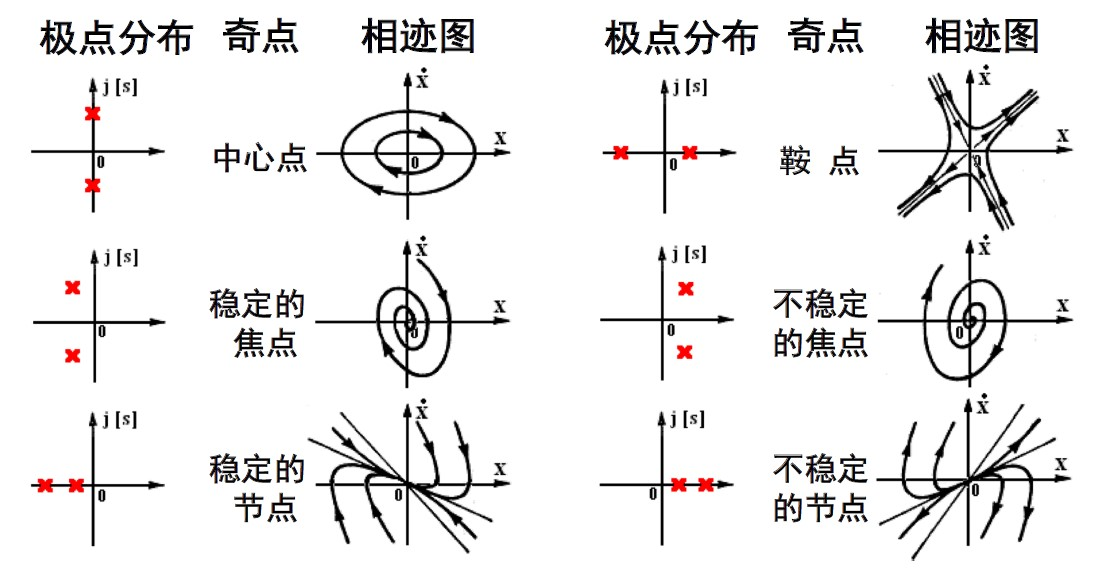
\includegraphics[width=\textwidth]{./figures/phasePlane.jpg} 
					\caption{线性二阶系统各种相轨迹}
					\label{fig:phaseplane}
				\end{figure}

		
	\newpage
	%% APPENDICES
	\appendix
	\section{常用公式}%
	\label{sec:常用公式}
		
			\paragraph{反正切函数性质}%
			\label{par:反正切函数性质}
				\ 	
				\begin{itemize}
					\item $\arctan A \pm \arctan B = \arctan \dfrac{A\pm B}{1\mp AB}$. 
				\end{itemize}

		\paragraph{渐进幅频特性分段函数公式}%
		\label{par:渐进幅频特性分段函数公式}
		
			\ 

			设开环传函为
			\[
				G(s) = \dfrac{K\prod\limits_{i=1}^{n}(\tau_i s+1)}{s^{v}\prod\limits_{j=1}^{m}(T_{j}s+1)} 
			,\] 
			其中 $\tau_{i-1}<\tau_i,\ T_{j-1}<T_j$. 
			则渐进幅频特性可表示为
			\[
				20\lg \left| G(\mathrm{j} \omega) \right| = 
				\begin{cases}
				\begin{aligned}
					20\left( \lg K - v\lg \omega \right)\quad, 1\le \omega < \min\left\{\dfrac{1}{\tau_1}, \dfrac{1}{T_1}\right\} \\
					20\left( \lg K - v\lg \omega - \sum_{j=1}^{k} \lg T_{j}\omega + \sum_{i=1}^{l} \lg \tau_{i}\omega  \right) ,\\
					\quad \min\left\{\dfrac{1}{\tau_l}, \dfrac{1}{T_k}\right\} \le \omega < \max\left\{\dfrac{1}{\tau_l}, \dfrac{1}{T_k} \right\}, \\
					\quad k=1,\ldots ,m,\ l=1,\ldots ,n \\

				\end{aligned}
				\end{cases}
			.\]
			
			\begin{nnr}  
				以上公式可理解为:先考虑积分环节,随后每到达一个转折频率就加上一项$\lg \dfrac{\omega}{\omega_i}$,该项符号取决于该转折频率是属于惯性环节还是微分环节,若是惯性环节为负,微分环节为正。
			\end{nnr} 
	
	\section{线性代数}%
	\label{sec:线性代数}
		
			\subsection{The Cayley-Hamilton Theorem}%
			\label{sub:the_cayley_hamilton_theorem}
			
				\begin{dfn}[``polynomial of a transformaiton'']  
				\label{dfn:_polynomial_of_a_transformaiton_}
				Let $f(x)=a_0+a_1x+\cdots +a_{n}x^{n}$ be a polynomial with coefficients from a field $\mathbb{F}$. Let $T$ be a linear operator on a vector space $V$ over $\mathbb{F}$. We define
				\[
					f(T) = a_0 I_V + a_1T + \cdots + a_{n}T^{n}
				,\]
				where $I_V$ is the identity linear operator, and $T^{n}$ is the $n$-fold composition of $T$, i.e. 
				\[
					T^{n} = T(T(\cdots T(x))\cdots ) \text{ for all } x\in V
				.\] 
				\end{dfn} 

				\begin{rmk}  
					Similarly, if a matrix $A\in M_{n\times n}(\mathbb{F})$, we define 
					\[
						f(A) = a_0 I_{n} + a_1A + \cdots  + a_{n} A^{n}
					.\] 
				\end{rmk} 

				\begin{nnt}[\textbf{The Cayley-Hamilton theorem}] 
				\label{the:ch}
					Let $T \,:\, V\to V$ be a linear transformation where $V$ is a finite-dimensional vector space over $\mathbb{F}$. Let $f(T)$ be the characteristic polynomial of $T$. Then, 
					\[
						f(T) = T_0
					\] 
					where $T_0$ is the zero transformation, i.e. $T_0(x)=0 \quad \forall x\in V$. In other words, $T$ satisfies its own characteristic equation.  
				\end{nnt} 

				\begin{nnc}[\textbf{Cayley-Hamilton theorem for matrices}] 
				\label{cor:ch_mtrx}
				Let $A\in M_{n\times n}(\mathbb{F})$, and let $f(t)$ be its characteristic polynomial. Then, 
				\[
					f(A) = \textbf{0}_{n\times n}
				.\] 
				\end{nnc} 
\end{document}
